\documentclass[12pt, a4paper]{report}
\usepackage[italian]{babel}
\usepackage[utf8]{inputenc}
\usepackage{amsmath, amsfonts, amssymb, amsthm}
\usepackage{graphicx, appendix, geometry}
\geometry{a4paper, top=2cm, bottom=3cm, left=2cm, right=2cm, bindingoffset=5mm}

\author{Athos Innocenti}
\title{\Huge Elettronica}\date{}\author{}
\begin{document}
\maketitle
\tableofcontents

\chapter{Semiconduttori e Diodi}
I \textbf{semiconduttori} sono materiali parzialmente conduttori cioè hanno una conducibilità più alta degli \textit{isolanti} (materiali \textit{dielettrici} in cui gli elettroni sono fissi in un reticolo quindi sono incapaci di muoversi e per questo non scorre corrente), ma minore dei \textit{conduttori} (tutti i \textit{metalli} nei quali, se si applica un potenziale, scorre corrente perché ci sono elettroni liberi disponibili all'interno del materiale). Tendenzialmente i semiconduttori sono degli isolanti, ma sotto opportune condizioni si comportano come conduttori. In questi materiali gli atomi sono legati tra loro tramite legami \textbf{covalenti} come nel caso dei materiali isolanti, con i quali condividono anche la dipendenza della conducibilità dalla \textit{temperatura}.
\begin{figure}[h]
\centering
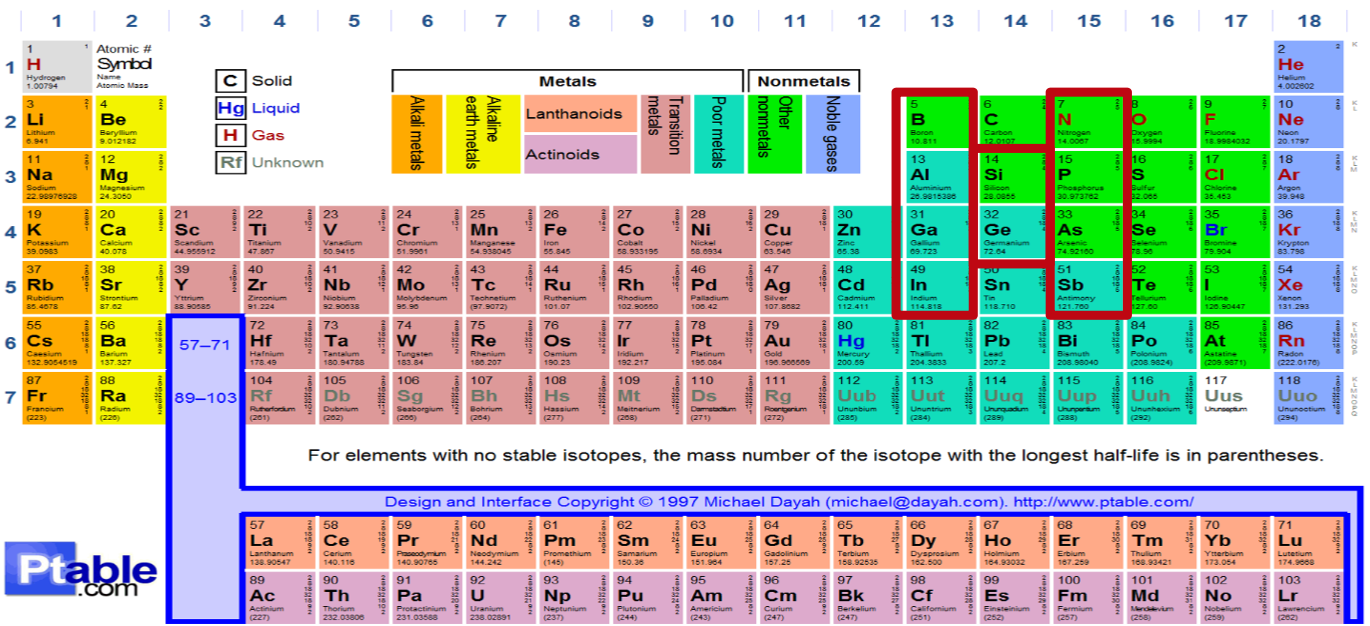
\includegraphics[scale=0.4,angle=0]{tavola_periodica.png}
\caption{Tavola periodica}
\end{figure}

I più comuni semiconduttori sono il \textbf{silicio} e il \textbf{germanio} che, trovandosi nella $IV^{a}$ colonna della tavola periodica, hanno quattro elettroni nell'orbitale più esterno. Sono gli unici semiconduttori \textbf{non composti}, cioè costituiti da atomi di un solo tipo. Altri possibili semiconduttori sono i seguenti composti \textbf{binari}: arseniuro di gallio GaAs, nitruro di gallio GaN, fosfuro di indio InP e il carburo di silicio SiC (un composto 4\,-\,4 perché sia il carbonio che il silicio appartengono alla quarta colonna), tutti formati da un elemento della $III^{a}$ colonna e da uno della $V^{a}$ e per questo si comportano come un elemento della quarta colonna (perché in media hanno quattro elettroni).\\Dunque, nei semiconduttori gli atomi coinvolti sono tutti collocati a cavallo della $IV^{a}$ colonna della tavola periodica: quella del carbonio (ma da solo non è usato come semiconduttore), silicio e germanio che hanno orbitali mezzi pieni e mezzi vuoti; cioè ci sono quattro elettroni e quattro spazi vuoti.

Di base, un materiale semiconduttore da solo è un materiale debolmente o per niente conduttore e non esprime, da solo, nessuna particolare proprietà, tuttavia diventa un materiale utilizzabile nel campo dell'elettronica quando viene \textbf{drogato}. Durante questo processo si parte da una matrice cristallina di materiale base che deve essere un materiale della quarta colonna, per esempio il silicio, e per \textbf{diffusione} si inserisce al suo interno una piccola quantità (circa una parte per miliardo) di \textbf{impurità}, ovvero di materiali appartenenti alla $III^{a}$ o alla $V^{a}$ colonna; generalmente sono rispettivamente il boro \textbf{B} e il fosforo \textbf{P}.

Nel caso del fosforo si parla di \textbf{impurità di quinta colonna} caratterizzata dall'avere un \textit{eccesso} di elettroni perché il fosforo ne ha cinque rispetto ai quattro del silicio. Il fosforo, inserito nella matrice di silicio, fornisce degli elettroni aggiuntivi (rappresentati tramite una carica negativa) rispetto al \textit{reticolo di base}, la struttura della matrice rimane la stessa, ovvero il reticolo del silicio, ma di tanto in tanto ci sono degli elettroni in più che rendono il materiale più \textbf{elettronegativo}, cioè più disponibile a fornire degli elettroni, e quindi si guadagna una certa conducibilità elettrica. In generale, quando si aggiunge un materiale \textit{drogante} di quinta colonna, il materiale che si ottiene è detto di \textbf{tipo n}. Quindi se il materiale di base è drogato da una impurità di tipo n significa che c'è un eccesso di elettroni, cioè di cariche negativa all'interno del materiale.

Nel caso del boro, o più in generale di un drogante di terza colonna, si parla di \textbf{impurità di terza colonna} caratterizzata dall'avere un \textit{difetto} di elettroni perché l'elemento di terza colonna ha solo tre elettroni rispetto ai quattro del reticolo. A livello pratico è come se per ogni impurità nella matrice si avesse un piccolo buco, cioè una mancanza di elettrone che prende il nome di \textbf{lacuna} e in genere si modella come se fosse una \textit{carica positiva}, infatti matematicamente le lacune vengono trattate come se fossero delle vere cariche positive per far tornare correttamente i conti. Il materiale ottenuto tramite questo secondo tipo di impurità è detto di \textbf{tipo p}.

Nell'interazione tra un materiale di tipo p e un materiale di tipo n si nota che gli elettroni in eccesso nel materiale di tipo n passano attraverso le lacune del materiale di tipo p.

Il drogaggio in entrambi i casi può essere fatto sia utilizzando un materiale \textbf{puro} come il silicio e il germanio, oppure tramite un materiale \textbf{composto}, l'importante è che il materiale sia mediamente di quarta colonna. Il silicio è di gran lunga il materiale più usato però non è strettamente quello che ma prestazioni migliori, il germanio viene maggiormente utilizzato per i dispositivi a radiofrequenza ma è molto più raro come lo sono anche GaAs, GaN e InP. SiC è costituito da carbonio e silicio che sono facilmente reperibili ma deve essere costruito quindi rimane comunque mediamente costoso.\\Lo specifico materiale da utilizzare dipende dall'elettronica che si deve andare a costruire. Per l'elettronica digitale, come celle logiche e microprocessori, si può utilizzare la tecnologia del silicio più i vari droganti. Per l'elettronica di potenza ad alte prestazioni si tende a preferire il nitruro di gallio o il carburo di silicio per le loro caratteristiche. Per i dispositivi optoelettronici, per esempio i LED, si usano invece il fosfuro di indio e l'arseniuro di gallio.

\section{Giunzioni PN}
Si ottengono quando si fa un drogaggio del silicio, cioè quando si aggiunge un materiale al silicio puro. L'aspetto particolare non è tanto il drogaggio del materiale di base quanto il mettere in contatto materiali drogati di tipo diverso, p ed n.

Nel caso dei materiali di tipo p si va a studiare il numero di \textbf{accettori}, indicato con $N_{a}$, rappresentante il numero di \textit{lacune} per unità di volume. Al contrario, per i materiali di tipo n si va a studiare il numero $N_{d}$ rappresentante il numero di \textbf{donatori} per unità di volume, cioè il numero di atomi che donano un elettrone. Sia $N_{a}$ che $N_{d}$ sono dell'ordine di $10^{-9}\,, 10^{-10}$ cioè un atomo ogni $10^{10}$ circa è un drogante di tipo p o n.

Più il silicio di base viene drogato e più esso tenderà a diventare un materiale con un comportamento sempre più lontano da quello del silicio di base. Di base il silicio si organizza in una \textit{matrice cristallina}, cioè come un \textit{cristallo} che non lascia passare lacune ed elettroni ma aggiungendo delle impurità si rendendo disponibili elettroni in più oppure delle lacune in cui potranno finire degli elettroni.

Per ottenere le \textbf{giunzioni p\,-\,n} si parte da una matrice di silicio la quale, tramite un processo di diffusione dall'alto, viene prima drogata con un drogante di tipo n andando a creare una \textit{tasca} e poi su una certa sezione già drogata della tasca viene ulteriormente inserito un drogante di tipo p (la diffusione può essere effettuata selettivamente in specifiche aree della matrice in base alle esigenze). La giunzione pn si formerà quindi lungo il \textit{bordo di confine} tra il drogaggio di tipo p e quello di tipo n.
\begin{figure}[ht]
\centering
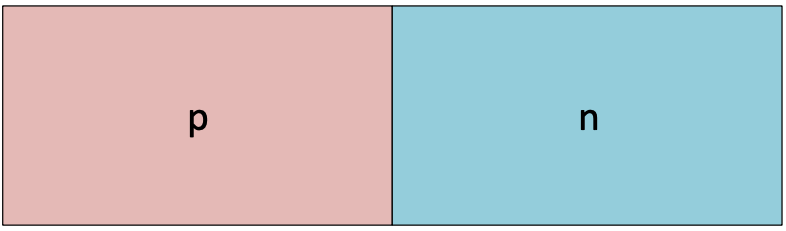
\includegraphics[scale=0.4,angle=0]{giunzione_pn.png}
\caption{Giunzione PN}
\end{figure}

Preso un materiale di tipo p avente un eccesso di lacune rispetto al reticolo e uno di tipo n con un eccesso di elettroni, nonostante le impurità i due materiali sono entrambi \textit{elettricamente neutri}. Lo sbilanciamento di elettroni in un lato e di lacune disponibili nell'altro fa sì che nel momento in cui un materiale di tipo p e uno di tipo n entrano in contatto si verifica un fenomeno di \textbf{migrazione} per cui statisticamente gli elettroni in eccesso nel materiale di tipo n tendono a migrare nel materiale di tipo p avente dello spazio libero dato dalle lacune.
\begin{figure}[h]
\centering
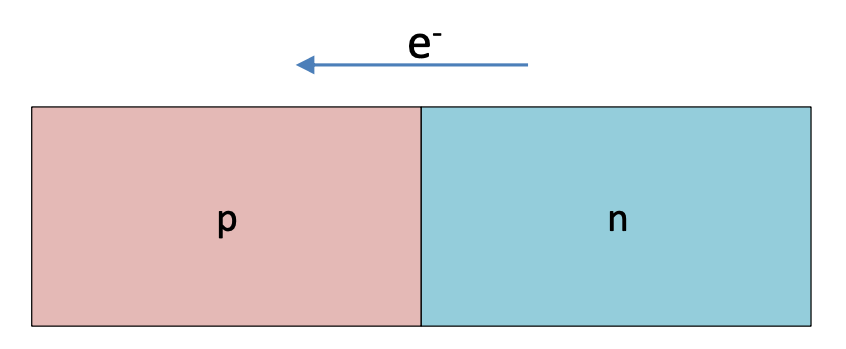
\includegraphics[scale=0.4,angle=0]{giunzione_pn_elettroni.png}
\caption{Migrazione degli elettroni}
\end{figure}

Via via che gli elettroni passano nel materiale di tipo p ognuno di essi si inserisce in una lacuna, riempiendola. Nel far ciò il materiale di tipo p passa dall'essere un materiale neutro (era un materiale della terza colonna con tre protoni e tre elettroni) ad essere \textit{negativamente carico} e questo comporta che la carica negativa che si è venuta a creare emette un \textbf{campo elettrico} che respinge altre cariche negative. Per cui, via via che gli elettroni passano nel materiale di tipo p tale materiale diventa più carico negativamente e si genera un campo elettrico negativo, inoltre gli elettroni che sono passati hanno liberato posti all'interno del materiale di tipo n nel quale quindi si crea una \textit{carica positiva}. Si arriva quindi ad un punto in cui sono passati un certo numero di elettroni che hanno generato un campo elettrico che impedisce ad altri elettroni nel materiale di tipo n di passare, si ha un \textbf{equilibrio}.

All'equilibrio, un certo numero di elettroni è passato nel materiale di tipo p e ha creato una zona a carica nettamente negativa e si sono formate un certo numero di lacune nel materiale di tipo n che hanno creato una zona a carica nettamente positiva. In queste condizioni, non è possibile far fluire ulteriori elettroni perché verrebbero respinti dal campo elettrico generato dagli elettroni passati in precedenza.
\begin{figure}[ht]
\centering
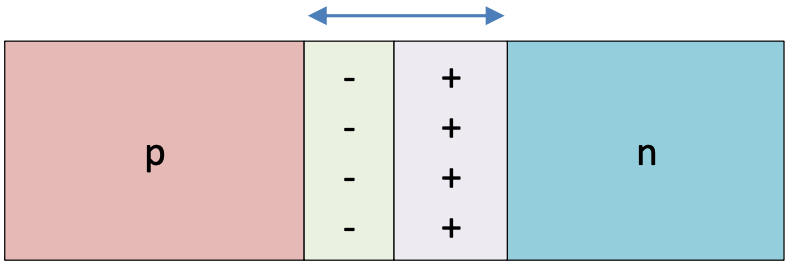
\includegraphics[scale=0.4,angle=0]{giunzione_pn_equilibrio.png}
\caption{Giunzione PN all'equilibrio}
\end{figure}

Nella zona a carica negativa non c'è più spazio per poter far arrivare e ospitare ulteriori elettroni e, analogamente, nella zona a carica positiva sono presenti tutti quegli atomi che in precedenza avevano cinque elettroni e ora ne hanno quattro, quindi non si possono più spostare altri elettroni perché si è tornati alla conformazione del reticolo cristallino del silicio con quattro elettroni; è silicio carico positivamente ma non ha elettroni trasferibili. Questo sbilanciamento di carica (da un lato una carica negativa netta e dall'altro una carica positiva netta) come già detto provoca un campo elettrico che blocca l'ulteriore diffusione di elettroni e la regione in cui sono presenti le due cariche nette opposte è chiamata \textbf{regione di svuotamento} o \textbf{regione di carica spaziale}. Di svuotamento nel senso che in quella regione sono stati eliminati tutti i \textit{portatori} di carica; di carica spaziale nel senso che questo procedimento ha portato a creare una \textit{densità di carica} positiva e negativa che implica la formazione di un campo elettrico.
\begin{figure}[h]
\centering
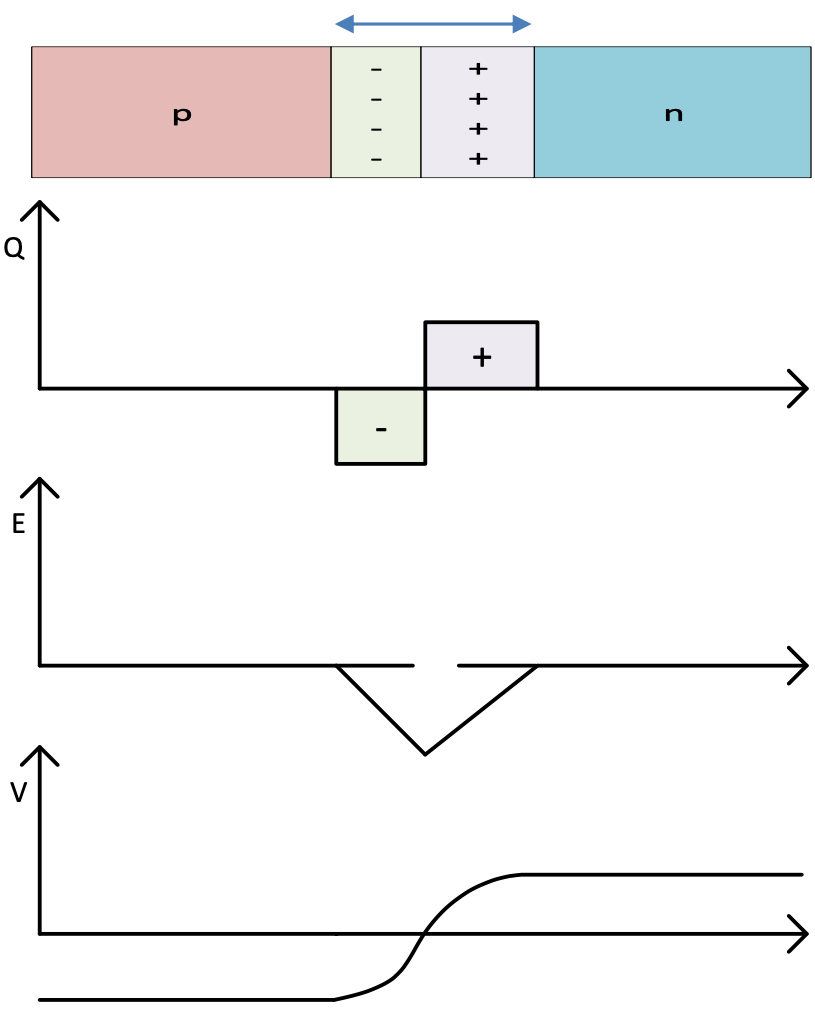
\includegraphics[scale=0.45,angle=0]{giunzione_pn_grafici.png}
\caption{Cariche, campo elettrico e potenziale della giunzione PN}
\label{grafici}
\end{figure}

Come si nota in figura \ref{grafici}, nel dominio della carica nella ragione di svuotamento relativa alla zona p si crea una regione di cariche nettamente negative mentre in quella relativa alla zona n se ne crea una di cariche nettamente positiva.

Dallo studio della carica è possibile ricavare informazioni relative sia al campo elettrico che al potenziale. Percorrendo l'asse \textit{x} da sinistra verso destra e integrando rispetto alle cariche incontrate, cioè integrando la \textit{distribuzione} di carica (la funzione rappresentata nel primo grafico - per semplicità si è presa esattamente rettangolare cioè una distribuzione uniforme), si ricava il campo elettrico $E(x) = \int q\,dx$ (secondo grafico di figura \ref{grafici}) che è una funzione decrescente nell'intervallo in cui ci sono solo cariche negative, ha il minimo in corrispondenza della giunzione pn e da lì diventa una funzione crescente dal momento in cui si entra nella zona con carica positiva netta. Sia la crescita che la decrescita sono entrambe \textit{lineari} avendo supposto una distribuzione uniforme in entrambe le zone. Inoltre la funzione $E(x)$ nei due estremi vale $0$ perché la quantità di carica positiva e negativa è \textit{la stessa} e questo è dovuto al fatto che ad ogni elettrone passato corrisponde una lacuna lasciata.

L'\textit{estensione} della zona a carica positiva e di quella a carica negativa non sono uguali perché l'estensione fisica della regione di svuotamento sia nel lato p che nel lato n è \textit{direttamente proporzionale} a quante lacune e a quanti elettroni ci sono per unità di volume. Si scambia la stessa quantità di elettroni e lacune ma la dimensione delle due zone dipende dalla quantità di portatori, cioè dipende dalla \textit{densità} del drogante. Se per esempio si suppone che il drogaggio della parte p sia il doppio di quello della parte n (quindi $N_{a} > N_{d}$), siccome il numero totale di elettroni è lo stesso a destra e a sinistra, una volta riempita tutta la regione di svuotamento si sa che ci sono $N_{a}$ elettroni per unità di volume nella zona costituente la carica negativa netta. Posta $x_p$ la lunghezza della zona a carica negativa netta e $x_{n}$ quella della zona a carica positiva netta, $N_{a} \cdot x_{p}$ rappresenta la quantità di elettroni nella zona p e deve essere uguale alla quantità di cariche positive nella zona n, cioè deve valere:
\begin{equation}
    N_{a} \cdot x_p = N_{d} \cdot x_n
    \label{giunzione_pn}
\end{equation}
che riassume il fatto che un elettrone che si sposta dalla zona n alla zona p lascia una carica positiva nella zona n e porta una carica negativa nella zona p e gli spazi utilizzabili sono quelli dovuti alle lacune e alle cariche negative che sono state create con il drogaggio. In base alla \eqref{giunzione_pn} l'estensione della regione di svuotamento è \textit{inversamente proporzionale} alla quantità di drogante: più la regione è drogata e più sarà sottile e viceversa. Questo significa ancora che nel primo grafico di figura \ref{grafici} i due rettangoli, aventi base $x_{p}$ e $x_{n}$ e altezza rispettivamente $N_{a}$ e $N_{d}$, devono avere la stessa area.

Integrando il campo elettrico $E(x)$ si ottiene il \textbf{potenziale} che, a meno di una costante presa negativa, parte negativo e diventa positivo, cioè nella zona n è più positivo che nella zona p (terzo grafico di figura \ref{grafici}).

\section{Diodi}
Il risultato finale di quanto detto è la creazione di un campo elettrico e di una differenza di potenziale, cioè una \textbf{tensione}, tra la zona n e la zona p. La differenza di potenziale fa sì che gli ulteriori elettroni che si trovano nella zona n (quindi non quelli che vanno a formare la carica positiva netta) siano bloccati e non possano passare nella zona p. Analogamente, anche le lacune non possono andare dalla zona p a quella n perché trovano un potenziale positivo e vengono quindi respinte. Ci si trova in una condizione di equilibrio. Il dispositivo così ottenuto è chiamato \textbf{diodo}; in particolare è un \textit{diodo a giunzione pn}.
\begin{figure}[h]
\centering
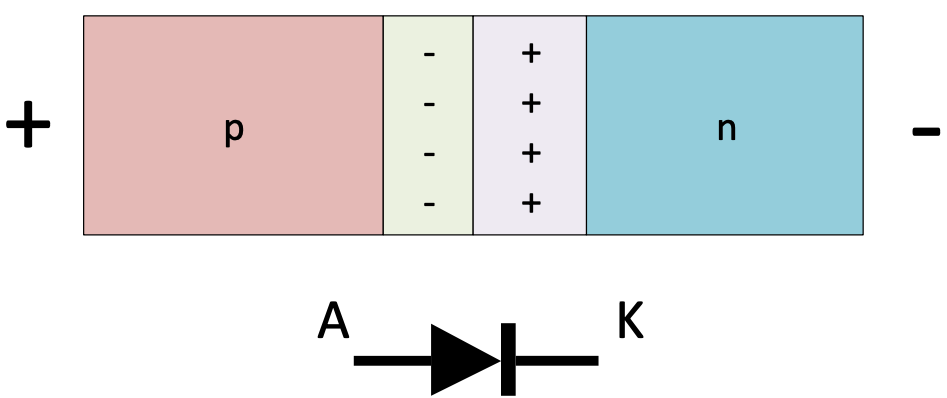
\includegraphics[scale=0.4,angle=0]{diodo.png}
\caption{Struttura e simbolo di un diodo in \textit{polarizzazione diretta}}
\end{figure}

Il diodo è formato da due terminali chiamati \textbf{anodo} e \textbf{catodo}, indicati con \textit{A} e \textit{K} e corrispondenti rispettivamente alla zona \textit{p} contente le lacune e alla zona \textit{n} contente gli elettroni. La freccia che compare nel simbolo del diodo indica il verso in cui scorre la \textit{corrente} (intesa come cariche positive): essa scorre dall'anodo verso il catodo. Se la corrente si muove dall'anodo verso il catodo significa che gli elettroni si spostano nel verso opposto: dal catodo all'anodo.

Come detto in precedenza, la barriera di potenziale che si viene a creare in corrispondenza delle due cariche nette e della giunzione impedisce agli elettroni di spostarsi dalla zona n alla zona p cioè dal catodo all'anodo. Tuttavia questo risulta essere vero fintanto che non si applica esternamente un certo \textit{potenziale}. In particolare, se si applica un potenziale \textit{positivo} all'anodo e \textit{negativo} al catodo ci si trova nelle condizioni di \textbf{polarizzazione diretta} tramite la quale il potenziale positivo applicato all'anodo fa alzare il potenziale della regione p e il potenziale negativo applicato al catodo fa abbassare il potenziale della regione n. Inoltre, fintanto che non c'è corrente all'interno della zona p non c'è caduta di potenziale, quindi il potenziale all'estrema sinistra è lo stesso potenziale del punto in cui inizia l'area con la carica negativa netta, lo stesso vale per la zona n. Con l'applicazione di potenziale esterno ai due estremi la curva tende a diventare sempre più piatta tendendo a diventare parallela all'asse \textit{x}; in queste condizioni gli elettroni e le lacune non incontrano più nessuna barriera di potenziale, quindi nessun ostacolo, e per questo sono liberi di fluire. Via via che si incrementa il potenziale in p e lo si abbassa in n, un po' di elettroni dal generatore esterno passano attraverso la zona n e vanno a neutralizzare la carica positiva netta. A questo punto, per effetto del \textit{bilanciamento} delle cariche, per ogni carica positiva che viene bilanciata a destra, un elettrone nella carica negativa netta si stacca e va verso il generatore passando attraverso la zona p e infine uscendo dal diodo Più questo processo va avanti e poi la regione di svuotamento diventa più stretta fino a svanire del tutto, una volta eliminata gli elettroni sono liberi di fluire.

Una volta raggiunta una certa tensione viene quindi annullata la barriera di potenziale e gli elettroni sono liberi di scorrere nel materiale pn. Dunque, applicando una tensione maggiore di una certa soglia inizia a scorrere corrente. Questa tensione soglia prende il nome di \textbf{tensione del diodo} (del potenziale interno che si era creato intorno alla giunzione pn con le due cariche nette opposte), viene indicata con $V_{D}$. Per un diodo al \textit{silicio} $V_D \approx 0,7\,V$, il che significa che se col generatore si supera la tensione di $0,7\,V$ si riesce ad annullare la barriera di potenziale nel mezzo del diodo pn e inizia a scorrere corrente con un andamento \textbf{esponenziale} con la tensione applicata al diodo:
\begin{equation}
    I_{D} = I_{0}\,(e^{(V_{D}/nV_{T})} - 1)
    \label{corrente_id}
\end{equation}
Per cui, fino a $0,7\,V$ non succede niente, superata tale soglia la corrente inizia a crescere esponenzialmente perché non incontra più nessun ostacolo.

Inizialmente si era detto che se non scorre corrente la parte di materiale p ed n non producono una caduta di tensione, però in realtà intrinsecamente le due parti di materiale p ed n sono anche \textit{conduttori} quindi presentano una loro certa \textbf{resistività}. Dunque se si volesse fare una rappresentazione veritiera del circuito, oltre al generatore e al diodo \textit{ideale} bisognerebbe aggiungere due \textbf{resistenze}: una lato anodo rappresentante la conducibilità del materiale p e una lato catodo rappresentante quella del materiale n. Da questa rappresentazione si può quindi vedere come nella realtà ai capi della giunzione arrivi meno tensione di quella effettiva. 

Sapendo che la tensione delle resistenze è data da $V = R \cdot I$, la curva è esponenziale un volta superata la soglia di $0,7\,V$ ma ad un certo punto la tensione che si genera per \textit{caduta resistiva} è così grande che la tensione ai capi del diodo non cresce più, a quel punto la corrente $I_{D}$ non sarà più esponenziale ma \textit{lineare}. Meno corrente il diodo è in grado di portare e tanto prima di entrerà nella regione a crescita lineare.

Nella norma la regione di tipo p e quella di tipo n non sono drogate in maniera omologa ma una delle due è molto più drogata dell'altra. Il più delle volte è la regione n ad essere più drogata della regione p, cioè vale che $N_{d} >> N_{a}$. In queste condizioni ci sono tanti portatori di tipo n nella zona n (inteso come densità) ma ci sono poche lacune nella zona p, quindi quando un elettrone passa nella zona p si trova in una sorta di mare deserto di lacune. Per questa situazione si parla di \textbf{portatori minoritari} intendo il fatto che i portatori, cioè le lacune, sono molto sparsi e questo comporta che si hanno fenomeni di diffusione degli elettroni nel lato p e sono fenomeni non simmetrici, cioè non si osservazione la stessa situazione anche per la lacune nel lato n. L'aspetto principale è che via via che nel diodo sono presenti elettroni, questi si vanno ad accumulare nella parte di tipo p causando un fenomeno detto di \textbf{accumulo di carica} che, si vedrà più avanti, ha un effetto indesiderato.
\\\\Le considerazioni fatte finora sono relative al caso di polarizzazione diretta in cui si applica un potenziale positivo all'anodo e uno negativo al catodo. Nel caso contrario, detto \textbf{polarizzazione inversa} in cui si applica un potenziale negativo all'anodo e uno positivo al catodo, riprendendo l'andamento del potenziale in figura \ref{grafici}, il potenziale negativo applicato all'anodo fa abbassare ulteriormente il potenziale della regione p e il potenziale positivo applicato al catodo fa alzare ancora di più il potenziale della regione n.
\begin{figure}[h]
\centering
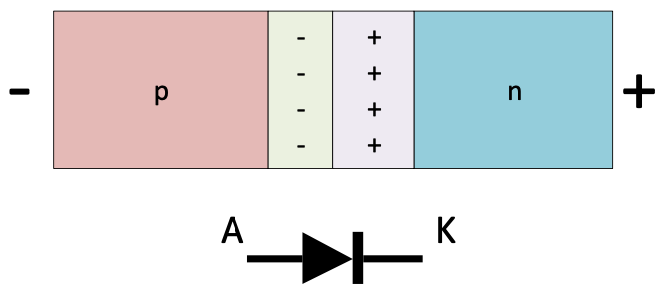
\includegraphics[scale=0.5,angle=0]{diodo_polarizzazione_inversa.png}
\caption{Diodo in \textit{polarizzazione inversa}}
\end{figure}
\\Questo comporta un aumento del valore assoluto della barriera di potenziale che diventerà più ripida. Inoltre, gli elettroni immessi nella zona p tramite il generatore esterno, si vanno ad aggiungere alla regione di svuotamento originale e, viceversa, nella zona n degli elettroni abbandonano la zona uscendo dal diodo. Il risultato netto è che la regione di svuotamento si \textit{allarga} con un corrispondente incremento della barriera di potenziale: i due rettangoli nel primo grafico di figura \ref{grafici} diventano più grandi, quindi aumenta anche il campo elettrico $E(x)$. Più aumenta la barriera di potenziale, più si accumulano cariche e più diventa difficile lo scorrimento della corrente attraverso il diodo. In realtà si ha comunque una corrente che scorre dal catodo all'anodo ed è definita dalla formula \eqref{corrente_id} che quindi vale sia per la polarizzazioni diretta che per quella inversa. In particolare, la corrente che scorre in polarizzazione inversa (anche detto \textbf{reverse bias}) è $I_{0}$ che è molto bassa (dell'ordine di $10^{-7} A$) ma comunque non nulla. Questa \textit{corrente di perdita} sarà tanto più piccola tanto più si sarà fatta attenzione nel progettare il diodo in modo tale che non ci sia e, generalmente, è proporzionale a quanta corrente può scorrere nel diodo nel caso di polarizzazione diretta o \textbf{forward bias}: diodi più grandi avranno corrente di perdita più grande e viceversa.

Il campo elettrico, come si vede nel secondo grafico di figura \ref{grafici}, ha il valore massimo in corrispondenza del confine tra la giunzione p e la giunzione n. In questo momento la parte centrale del diodo si comporta come un materiale \textbf{dielettrico} perché non conduce corrente a causa del fatto che le cariche sono tutte bloccate nella regione di svuotamento. Ma un materiale dielettrico non conduce corrente fino a quando non si supera la sua \textbf{rigidità dielettrica}. Il silicio ha un limite di rigidità dielettrica oltre la quale il materiale si \textit{rompe} (si dice che va in \textbf{breakdown}): il campo elettrico è così forte che le cariche elettriche da una parte vengono tirate dalla parte opposta fino ad essere \textit{strappate} dal reticolo cristallino e, a quel punto, inizia a scorrere corrente. Quindi il diodo, che in polarizzazione inversa non fa quasi scorrere corrente, una volta superata una certa soglia di rigidità dielettrica, detta \textbf{tensione di breakdown}, va in breakdown e da quel momento inizia a scorrere una corrente che cresce in maniera illimitata e improvvisa.
\begin{figure}[h]
\centering
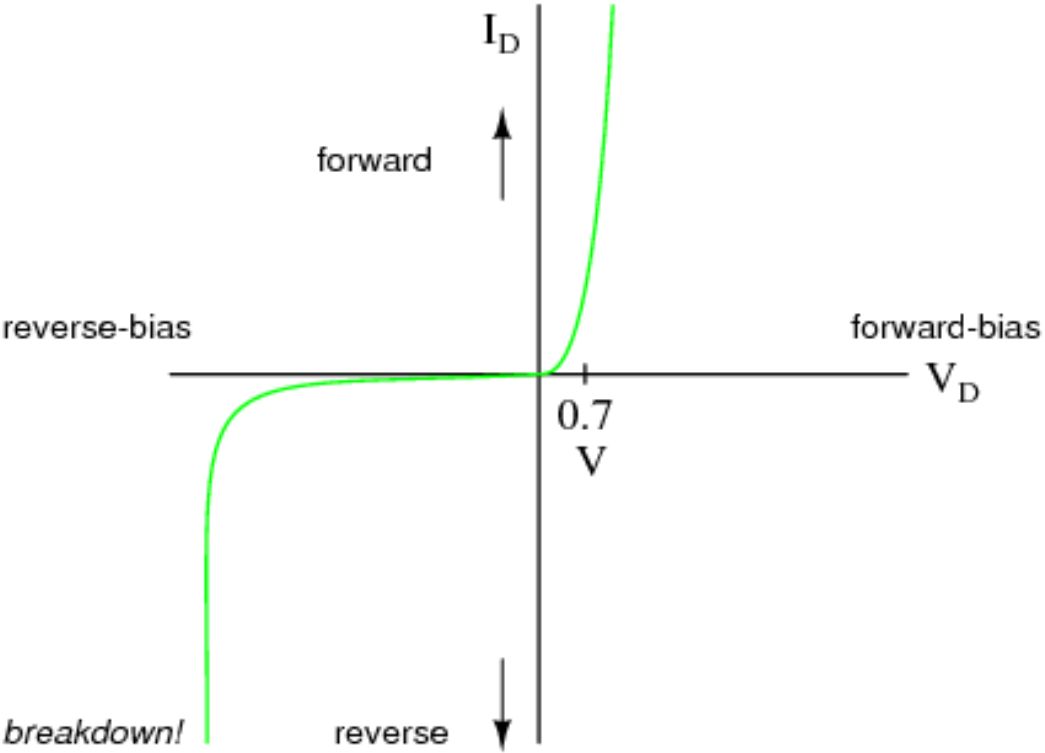
\includegraphics[scale=0.45,angle=0]{corrente_id.png}
\caption{Andamento della corrente nel diodo in polarizzazione diretta e inversa}
\end{figure}

In base a come sono costruiti diodo e circuito, il breakdown può essere \textit{reversibile}. Se all'interno del circuito (considerando un generatore ideale) la corrente non viene limitata in qualche modo (per esempio tramite delle resistenze) il diodo non è recuperabile dopo il breakdown. Ci sono due categorie di diodi: i diodi costruiti per andare in breakdown e quelli costruiti per non andarci; questi ultimi è molto probabile che effettivamente si rompano se vanno in breakdown indipendentemente dalla corrente. I diodi che invece sono costruiti appositamente per andare in breakdown sono chiamati \textbf{diodi Zener} e non si danneggiano andando in breakdown ma bisogna comunque limitare la corrente per esempio con una resistenza in serie per avere un corrente quasi lineare e quindi facilmente controllabile.
\begin{figure}[h]
\centering
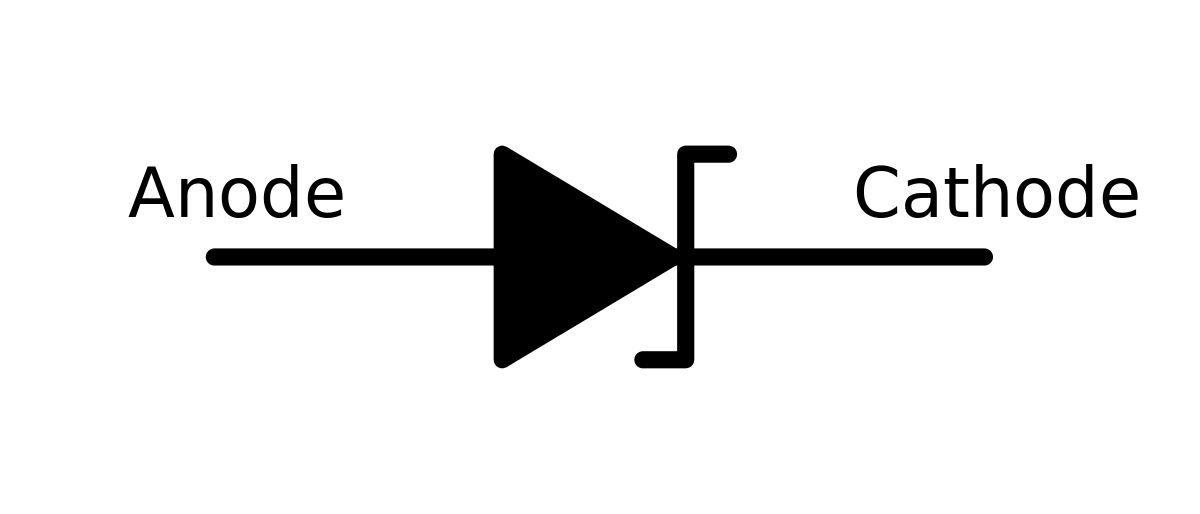
\includegraphics[scale=0.15,angle=0]{diodo_zener.png}
\caption{Simbolo del diodo Zener}
\end{figure}
\\In passato venivano usati per controllare la tensione ed è l'unico diodo che sopporta il breakdown inverso ma bisogna inserire una \textit{resistenza di limitazione}.\\

Nel contesto dell'elettronica digitale, in logica binaria, per una tensione $V_{D}$ compresa tra $0\,V$ e $0,7\,V$ si considera una corrente di $0\,A$ mentre oltre gli $0,7\,V$ si considera una corrente di $1\,A$, cioè infinita. Per tensioni negative, per $V_{D}$ compresa tra $0\,V$ e la tensione di breakdown si considera una corrente di $0\,A$ e oltre la tensione di breakdown si considera corrente infinitamente negativa. Nella realtà però il diodo è un dispositivo analogico caratterizzato da non avere cambi repentini di intensità di corrente.

\section{Diodi speciali}
Oltre al diodo Zener e ai diodi pn al silicio che si usano per controllare il verso di scorrimento della corrente, ci sono altre tipologie di diodi costruibili sfruttando ancora le proprietà dei materiali semiconduttori.
\begin{description}
    \item[Fotodiodo] È un dispositivo optoelettronico, cioè un dispositivo che sfrutta il dualismo tra energia e lunghezza d'onda (cioè tra fotone e l'energia che esso porta) per far sì che nel dispositivo a semiconduttore la luce che incide sul dispositivo stesso possa produrre degli effetti. A differenza di altri dispositivi optoelettronici che sono neri per non modificare il loro funzionamento a causa della luce, il fotodiodo è \textit{trasparente}. Il principio di funzionamento è del tutto analogo a quello della cella fotovoltaica: viene emessa corrente quando della luce incide sul fotodiodo. Per usarlo lo si polarizza in inversa e se della luce lo colpisce, se il fotone colpisce la regione di svuotamento, l'energia associata al fotone $e = \hbar \cdot \nu$ (con $\nu$ l'inverso della lunghezza d'onda) è in grado di prendere un elettrone nel reticolo cristallino e portarlo dalla \textbf{banda di valenza} nella \textbf{banda di conduzione} così che l'elettrone si stacca dalla sua lacuna, si crea una coppia elettone-lacuna liberi che è in grado di seguire il campo elettrico che si è creato tramite il quale la corrente scorre verso l'anodo, e si ha un passaggio di corrente. Quindi il diodo, che di base in polarizzazione inversa non conduce corrente, quando viene illuminato da una luce che abbia sufficiente energia per poter far passare gli elettroni dalla banda di valenza a quella di conduzione riesce a condurre corrente anche in condizioni di polarizzazione inversa. Si può usare per rilevare una radiazione luminosa incidente (per esempio in un telecomando a raggi infrarossi) oppure nei pannelli fotovoltaici in cui il pannello non è altro che un grande diodo pn al silicio e quando su di esso incide della luce solare diventa lui stesso un generatore di corrente con la corrente positiva uscente dall'anodo e la tensione che si genera ai capi del diodo che è sicuramente \textit{minore o uguale} della tensione di soglia del diodo stesso. Se la tensione che si genera fosse maggiore di $0,7\,V$ il diodo si polarizzerebbe direttamente e al suo interno vorrebbe scorrere una corrente contraria, dall'anodo al catodo. Normalmente una diodo al silicio per applicazioni fotovoltaiche genera tra gli $0,5$ e gli $0,6$ volt.
    \item[LED - Light Emitting Diode] Anche questo è un dispositivo optoelettronico che sostanzialmente ha un funzionamento opposto a quello del fotodiodo. È un dispositivo costruito in modo tale che quando viene polarizzato direttamente sia facile che nella regione di svuotamento si vadano a ricombinare elettroni e lacune; cioè è costruito in modo tale che gli elettroni che sono in banda di conduzione possano cadere in banda di valenza, così da poter liberare un fotone. La lunghezza d'onda del fotone liberato è \textit{inversamente proporzionale} all'energia (quindi la frequenza della radiazione luminosa emessa è direttamente proporzionale all'energia), quindi ad un salto energetico molto alto (barriera di potenziale alta) corrisponderà una lunghezza d'onda molto bassa cioè l'emissione del diodo si sposta verso gli ultravioletti; al contrario, se la barriera di potenziale è bassa l'emissione si sposta verso gli infrarossi. Accanto agli infrarossi c'è il \textit{rosso}, accanto agli ultravioletti c'è il \textit{viola}, nel mezzo partendo dal viola ci sono il blu, il verde, il giallo, l'arancione e infine il rosso. Dunque la lunghezza d'onda della luce emessa dal LED è esattamente determinata dalla sua distanza tra la banda di valenza e quella di conduzione, e a sua volta quella distanza è proporzionata dalla tensione che cade sul diodo, per questo il diodo LED è un diodo che normalmente ha una tensione di soglia \textit{molto alta}, soprattutto nel visibile e nell'ultravioletto. Inoltre, la tensione che cade ai capi del diodo, proprio perché è fatto per avere una barriera di potenziale grande, è tendenzialmente $> 1,5\,V$: per i LED \textit{rossi} è tipicamente $1,5\,V$, per i \textit{verdi} circa $1,8\,V$, per quelli \textit{blu} circa $2,2\,V$, per i diodi \textit{ultravioletti} è intorno ai $3\,V$, per i diodi \textit{infrarossi}, in particolare quelli nel vicino infrarosso, è circa $1,2\,V$. In ogni caso, la caduta di potenziale è proporzionata all'energia dell'emissione luminosa e tanto più l'emissione luminosa si sposta verso gli ultravioletti, tanto più è energetica e quindi tanto maggiore è la caduta di potenziale ai capi del diodo.
    \item[Diodo Shottky] Diodo particolare in cui la giunzione pn è fatta da un \textit{metallo} (per esempio l'\textit{alluminio} che è un materiale di $III^{a}$ colonna) nella zona p e da un \textit{semiconduttore} nella zona n. Questo accoppiamento fa sì che la regione di svuotamento si estenda solo nel lato del semiconduttore, nel metallo non esiste la regione di svuotamento perché la strutta molecolare di un metallo è il \textbf{mare di elettroni} in cui gli elettroni sono sempre liberi di muoversi: non si crea la regione di svuotamento ma il campo elettrico si. Questa caratteristica permette di avere una tensione di soglia \textit{minore} di quella di un diodo al silicio perché di fatto la regione di svuotamento è la metà di quella che si avrebbe normalmente. Come detto, mentre scorre corrente in un diodo normale si accumulano cariche minoritarie nella parte p.
    \begin{figure}[ht]
        \centering
        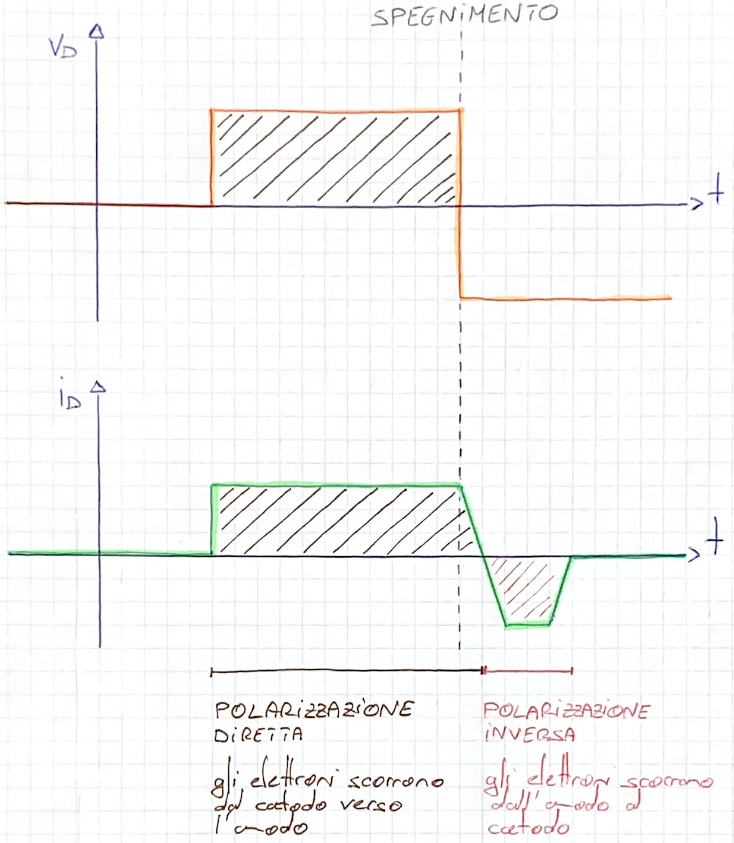
\includegraphics[scale=0.45,angle=0]{diodo_spegnimento.png}
        \caption{$V_{D}$ e $I_{D}$ di un diodo normale allo spegnimento}
    \end{figure}
    \\Questo comporta che quando si vuole spegnere il diodo, quindi $V_{D}$ diventa negativa perché si fa una polarizzazione inversa, esso si spegne lentamente, cioè $I_{D}$ scende lentamente ala valore previsto nel caso statico (invece si accende facilmente non appena viene polarizzato) perché ha accumulato cariche nella parte p che lo tengono ancora acceso. La corrente $I_{D}$ passa dall'essere positiva all'essere negativa per un certo tempo, fintanto che gli elettroni accumulati non vengono liberati. Indipendentemente dalla polarizzazione, passa comunque corrente. Tutto questo non succede nel diodo Shottky in cui, poiché la carica netta nella parte p non esiste, non esiste un accumulo di cariche bloccate nelle lacune e questo fa sì che quando il diodo passa in polarizzazione inversa si spegne immediatamente, cioè si comporta dinamicamente come un diodo ideale.
\end{description}

\chapter{BJT}
Il \textbf{BJT} viene così chiamato perché è un transistor bipolare, cioè composto da due poli. È un dispositivo a tre \textit{terminali} formato due due giunzioni: una giunzione np e una pn. I tre terminali sono: l'\textbf{emettitore} E, che costituisce la prima regione n a sinistra; la \textbf{base} B, corrispondente all'unica regione p presente e collocata nel mezzo; e infine il \textbf{collettore} C che invece è la seconda regione n collocata sulla destra del BJT.
\begin{figure}[h]
    \centering
    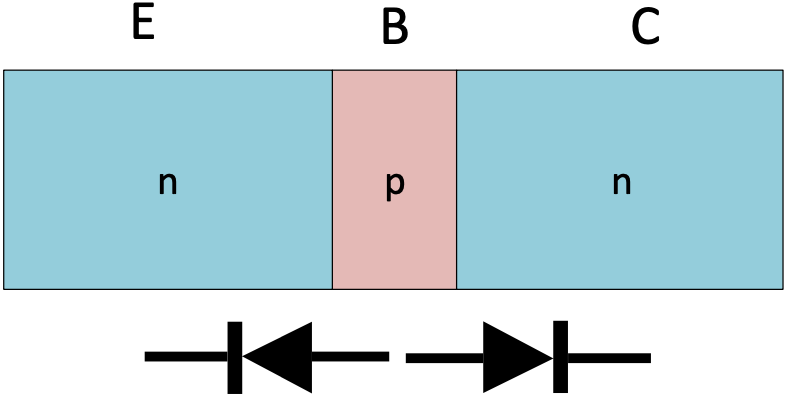
\includegraphics[scale=0.4,angle=0]{bjt_iniziale.png}
    \caption{Composizione di un BJT di tipo \textit{npn}}
    \label{bjt}
\end{figure}

Dalla rappresentazione schematica il BJT sembra un dispositivo simmetrico ma in realtà non lo è. Un aspetto importante è che la base è \textit{più stretta} dell'emettitore e del collettore, fondamentale per il suo funzionamento. Se fosse effettivamente costruito collegando due diodi in modo tale che le due zone p si tocchino, il dispositivo ottenuto non sarebbe un transistor perché due diodi così disposti, per l'equazione \eqref{giunzione_pn}, non producono nessun effetto perché non può scorrere corrente dall'emettitore al collettore in quanto è bloccata dal diodo np (emettitore - base) in quanto sarebbe polarizzato inversamente e analogamente non può scorrere corrente dal collettore all'emettitore perché bloccata dal diodo pn (base - collettore) polarizzato inversamente. Lo stesso vale nel caso di un BJT di tipo \textit{pnp}.
\begin{figure}[h]
    \centering
    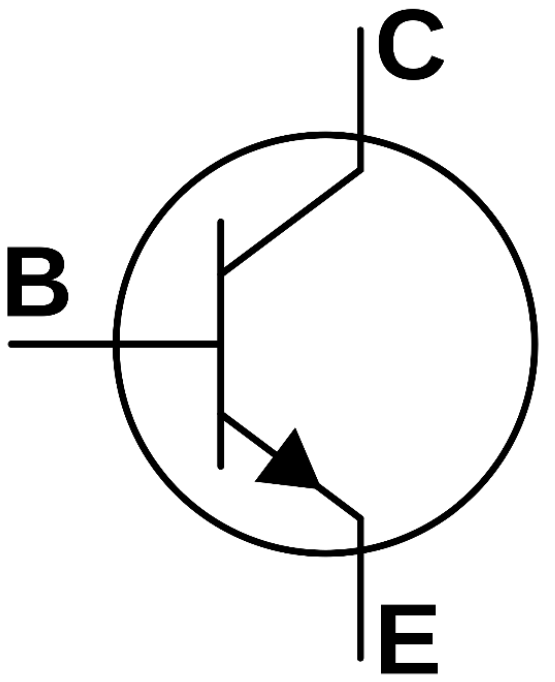
\includegraphics[scale=0.3,angle=0]{bjt_simbolo.png}
    \caption{Simbolo circuitale del BJT \textit{npn}}
\end{figure}

Nel simbolo circuitale del BJT la freccia indica la giunzione tra la base e l'emettitore. Nel caso del diodo classico a due terminali si prende \textit{positiva} la tensione dell'anodo e \textit{negativa} quella del catodo (quindi la tensione del diodo viene considerata positiva quando la tensione dell'anodo è positiva, ovvero il diodo è polarizzato direttamente); per il BJT si definiscono tre tensioni:
\begin{itemize}
    \item[$V_{be}$]: la tensione tra l'emettitore e la base che formano una giunzione pn. È \textit{positiva} quando la base è positiva rispetto all'emettitore perché $V_{be}$ è la differenza tra il potenziale (o tensione) della base $V_{b}$ (dove punta la freccia in figura \ref{tensioni_bjt}) e il potenziale dell'emettitore $V_{e}$ (dove parte la freccia). Quindi $V_{be} > 0$ significa che la giunzione tra emettitore e base è polarizzata \textit{direttamente}
    \item[$V_{bc}$]: la tensione tra la base e il collettore, è \textit{positiva} quando $V_{b} > V_{c}$ perché definita come differenza tra i potenziali $V_{b}$ e $V_{c}$
    \item[$V_{ce}$]: la tensione tra collettore ed emettitore, è \textit{positiva} quando $V_{c} > V_{e}$ perché definita come differenza tra i potenziali $V_{c}$ e $V_{e}$
\end{itemize}
\begin{figure}[h]
    \centering
    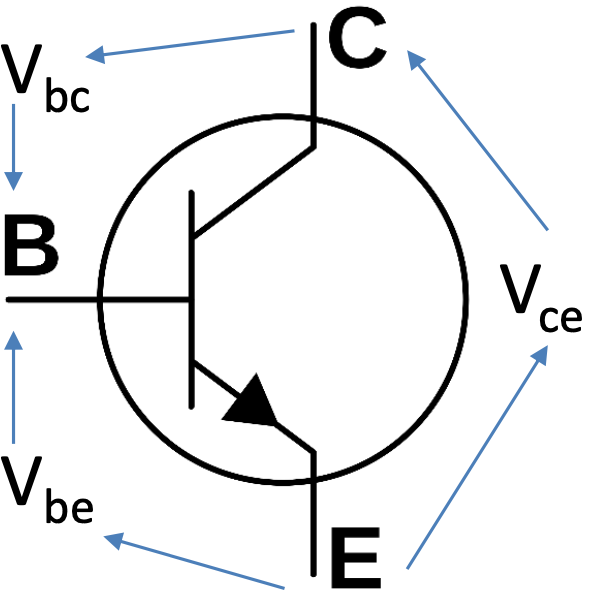
\includegraphics[scale=0.4,angle=0]{bjt_tensioni.png}
    \caption{Tensioni nel BJT \textit{npn}}
    \label{tensioni_bjt}
\end{figure}
Analogamente si hanno anche tre correnti, una per ognuno dei tre terminali del BJT:
\begin{itemize}
    \item[$I_{c}$]: la corrente del collettore, si prende \textit{positiva} quando è \textit{entrante} nel dispositivo
    \item[$I_{b}$]: la corrente di base, si prende \textit{positiva} quando è \textit{entrante} nel dispositivo
    \item[$I_{e}$]: la corrente dell'emettitore, si prende \textit{positiva} quando è \textit{uscente} nel dispositivo
\end{itemize}
Vale il principio di Kirchhoff per cui $I_{c} + I_{b} = I_{e}$.
\begin{figure}[h]
    \centering
    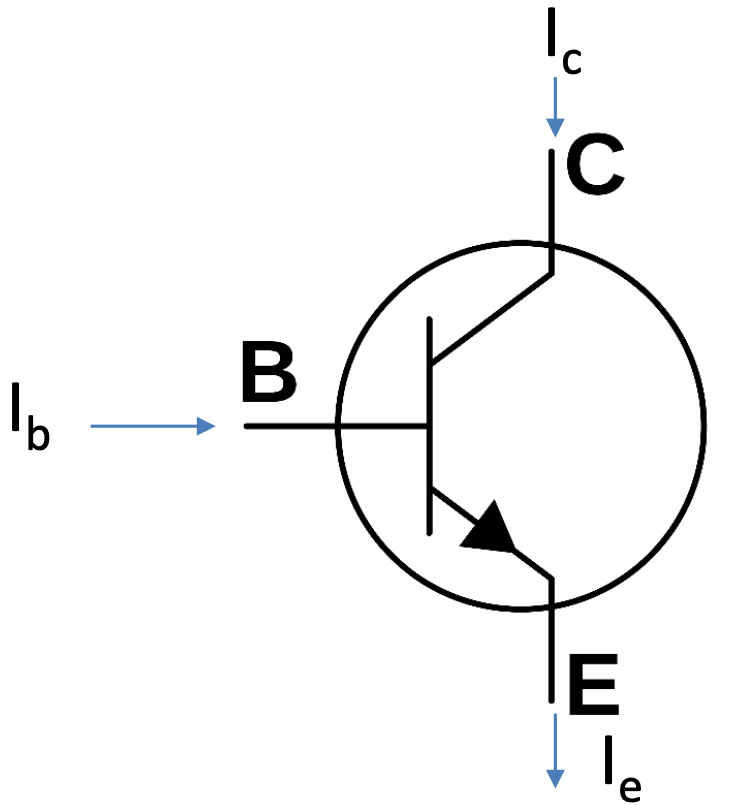
\includegraphics[scale=0.35,angle=0]{bjt_correnti.png}
    \caption{Correnti nel BJT \textit{npn}}
\end{figure}

\section{Regioni operative}
Il BJT è un dispositivo che può lavorare in \textit{quattro} modalità chiamate \textbf{regioni operative}: la regione di \textbf{cutoff} o \textbf{interdizione} in cui semplicemente il dispositivo è \textit{spento} e non sta facendo niente; la regione \textbf{attiva diretta}; la regione di \textbf{saturazione} e la regione \textbf{attiva inversa}. In tutte le regioni eccetto quella di cutoff il dispositivo fa qualcosa.

Si dice che il BJT è un \textbf{generatore di corrente controllato in corrente}, cioè le regioni di funzionamento sono determinate dalle correnti e/o dalle tensioni; in particolare ciò che guida il dispositivo è la corrente che entra in base $I_{b}$.

\subsection{Cutoff}
Nella regione di cutoff il transistor è spento, non passa corrente dal collettore all'emettitore. In questo caso \textit{entrambe} le giunzioni pn, BE tra la base e l'emettitore e BC tra la base e il collettore, sono polarizzate \textit{inversamente}, cioè sono in \textit{reverse bias}. Questo significa che:
\begin{equation*}
    V_{be} < V_{th} \text{ \, \, } V_{bc} < 0
\end{equation*}
con $V_{th}$ la tensione di soglia (anche detta potenziale di base). Per avere polarizzazione inversa tra base e collettore, il collettore deve avere un potenziale $V_{c}$ più alto rispetto al potenziale di base $V_{b}$. Questo succede finché il collettore non arriva ad avere un potenziale al massimo inferiore di $0,5\,V$ rispetto alla tensione di base, quindi o è una tensione molto elevata oppure è una tensione vicina alla tensione di base $V_{th}$ ma non sotto $0,5\,V$ rispetto a $V_{th}$ altrimenti si polarizzerebbe direttamente. Per le correnti, nella regione di cutoff si ha:
\begin{equation*}
    I_{b} = 0\,A \text{ \, \, } I_{c} = 0\,A
\end{equation*}
In realtà più che $0\,A$ sarà uguale ad una piccola corrente di perdita $I_{0}$ che è la corrente inversa della giunzione pn che si sta considerando.
\begin{figure}[h]
    \centering
    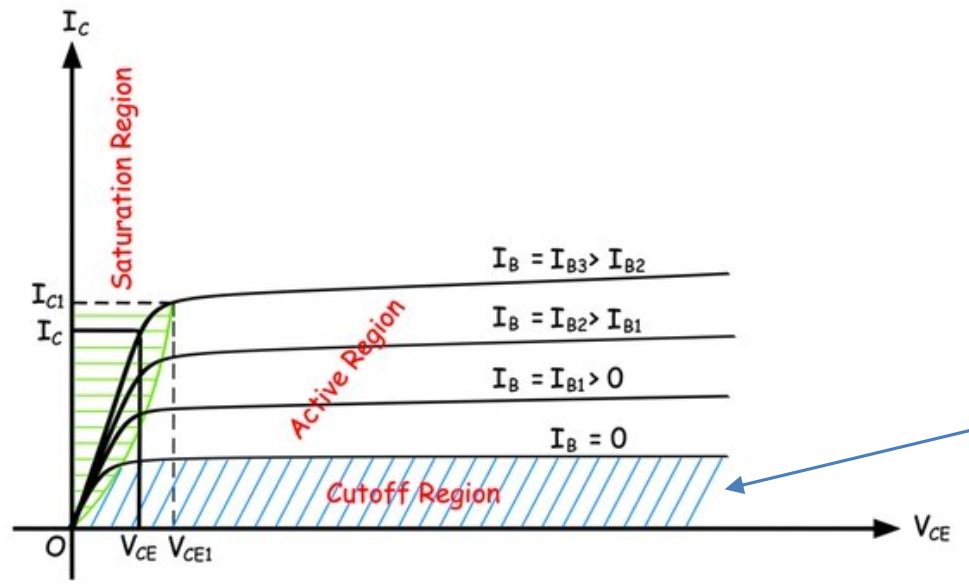
\includegraphics[scale=0.4,angle=0]{bjt_cutoff.png}
    \caption{Regione di cutoff}
\end{figure}

I grafici dei transistors hanno normalmente $V_{ce}$ nelle ascisse, $I_{c}$ nelle ordinate e le curve vengono disegnate al variare della \textit{variabile di controllo} che è $I_{b}$. Nella regione di cutoff si ha, come detto, $I_{b} = 0\,A$ e $I_{c} \approx I_{0}$ che è una corrente molto piccola.
\subsection{Attiva diretta}
Nella regione attiva diretta la giunzione BE tra la base e l'emettitore è polarizzata \textit{direttamente} quindi:
\begin{equation*}
    V_{be} > V_{th} \text{ \, \, } I_{b} > 0
\end{equation*}
La giunzione BC tra la base e il collettore è invece in polarizzazione \textit{inversa}:
\begin{equation*}
    V_{bc} < 0
\end{equation*}
cioè il potenziale del collettore è alto, maggiore di quello della base. Sotto queste condizioni ($I_{b} > 0 $ e $V_{bc} < 0$) il dispositivo si comporta come un transistor, cioè come un generatore di corrente controllato in corrente:
\begin{equation}
    I_{c} = h_{fe} \cdot I_{b}
    \label{corrente_attiva_diretta}
\end{equation}
dove $h_{fe}$ è una costante il cui valore è normalmente molto maggiore di zero (dell'ordine delle decine o centinaia) ed è chiamata \textbf{guadagno in corrente} del transistor. Dunque, la polarizzazione diretta della giunzione BE fa sì che scorra corrente dalla base all'emettitore (ovvero elettroni dall'emettitore alla base) e la polarizzazione inversa della giunzione BC alza il potenziale del collettore facendo sì che scorra una corrente molto maggiore dal collettore all'emettitore.
\begin{figure}[h]
    \centering
    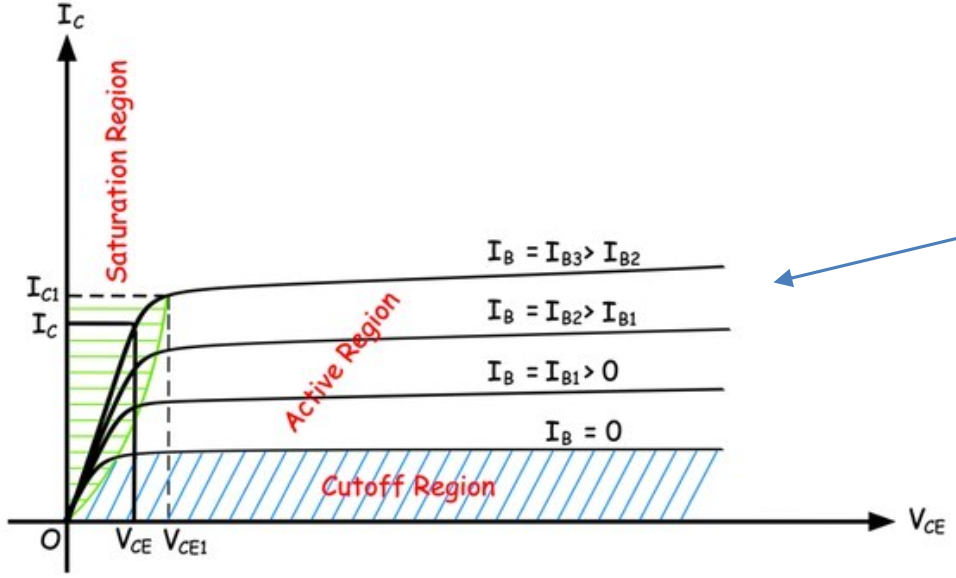
\includegraphics[scale=0.4,angle=0]{bjt_attiva_diretta.png}
    \caption{Regione attiva diretta}
    \label{attiva_diretta}
\end{figure}

Si è detto inizialmente che la base del BJT è più stretta rispetto agli altri due terminali. Polarizzando direttamente BE si crea un potenziale positivo nella base $V_{b} > 0$ e negativo nell'emettitore $V_{e} < 0$, quindi scorre corrente dalla base verso l'emettitore ed elettroni dall'emettitore alla base. Inoltre, la tensione del collettore è molto maggiore di quella di base $V_{c} >> V_{b}$ quindi la giunzione pn BC è polarizzata inversamente. Normalmente la giunzione BC sarebbe un diodo, quindi non ci sarebbero elettroni disponibili nella regione p della base per andare nella regione n del collettore perché tra le due c'è una regione di svuotamento e c'è una differenza di potenziale. Il fatto che la base sia molto stretta, che il potenziale del collettore sia molto elevato e che l'emettitore stia emettendo elettroni verso la base fa sì che nel momento in cui un elettrone passa dall'emettitore alla base tale elettrone diventa disponibile (nella zona p c'è scarsità di elettroni) e, grazie al potenziale molto elevato dal collettore, viene attirato e trasportato nella regione del collettore e da lì risale nella corrente arrivando fino al collettore stesso. Quindi gli elettroni della giunzione BE, che erano destinati a rientrare verso la base come avviene in una qualsiasi giunzione pn, in realtà prima di ricombinarsi vengono catturati dal campo elettrico del collettore che li strappa dalla ricombinazione così da saltare la base e andare direttamente nella regione n del collettore. In un transistor la base viene quindi fatta sottile per evitare la ricombinazione degli elettroni nella base in modo che vadano invece nel collettore.

Tutto questo processo è \textit{ragionevolmente efficiente} il che vuol dire che una percentuale molto elevata degli elettroni (per esempio 99 elettroni su 100) provenienti dall'emettitore salta la base per andare nell'emettitore e solo una piccola percentuale si ferma nella base, ovvero:
\begin{equation*}
    \frac{I_{c}}{I_{b}} \approx 99
\end{equation*}
cioè 99 elettroni vanno nel collettore e 1 nella base. Il guadagno in corrente del transistor è:
\begin{equation*}
    \frac{I_{e}}{I_{b}} \approx 100
\end{equation*}
Se il guadagno del transistor fosse 50 significa che 2 elettroni rimangono in base e 98 vanno nel collettore. I guadagni medi dei transistor sono molto elevati.

Tutto questo processo però finisce nel momento in cui non c'è più un sufficiente potenziale nel collettore per attirare gli elettroni. A quel punto gli elettroni rimangono all'interno della base, si ricombinano e si passa alla saturazione. 

Per una tensione del collettore abbastanza elevata (quindi per $V_{ce}$ grande) la corrente del collettore $I_{c}$ è \textit{lineare} (regione attiva diretta - figura \ref{attiva_diretta}), ma nel momento in cui il potenziale del collettore diventa piccolo la corrente del collettore tende a zero (regione di saturazione - figura \ref{saturazione}). Sotto un certo livello di tensione del collettore, che si prende intorno ai $ 0,2 - 0,3\,V$, si considera il dispositivo come in saturazione.

\subsection{Saturazione}
Nella regione di saturazione sia la giunzione tra la base e l'emettitore che quella tra la base e il collettore sono \textit{entrambe} in  polarizzazione \textit{diretta}. A differenza del caso precedente in cui il potenziale del collettore era molto elevato e per questo $V_{bc} < 0$ e poteva scorrere molta corrente secondo l'equazione \eqref{corrente_attiva_diretta}, adesso si abbassa il potenziale del collettore a circa $ 0,2 - 0,3\,V$ quindi inferiore al potenziale della base. Quindi la giunzione BC è polarizzata direttamente perché la tensione del collettore è circa $0,2\,V$, quella della base è di $0,8\,V$ e dunque $V_{bc} = 0,6\,V$. Tutto questo comporta che la corrente del collettore diminuisce e diventa minore strettamente della massima possibile in regione attiva diretta, cioè:
\begin{equation*}
    I_{c} < h_{fe} \cdot I_{b}
\end{equation*}
Si dice che il transistor \textit{ha saturato} cioè la tensione del collettore $V_{c}$ è diventata così bassa che non è più in grado di far scorrere le cariche. Per il resto, si ha:
\begin{equation*}
    V_{be} > V_{th} \text{ \, \, } V_{ce} < V_{ce-sat} \text{ \, \, } I_{b} > 0
\end{equation*}
\begin{figure}[h]
    \centering
    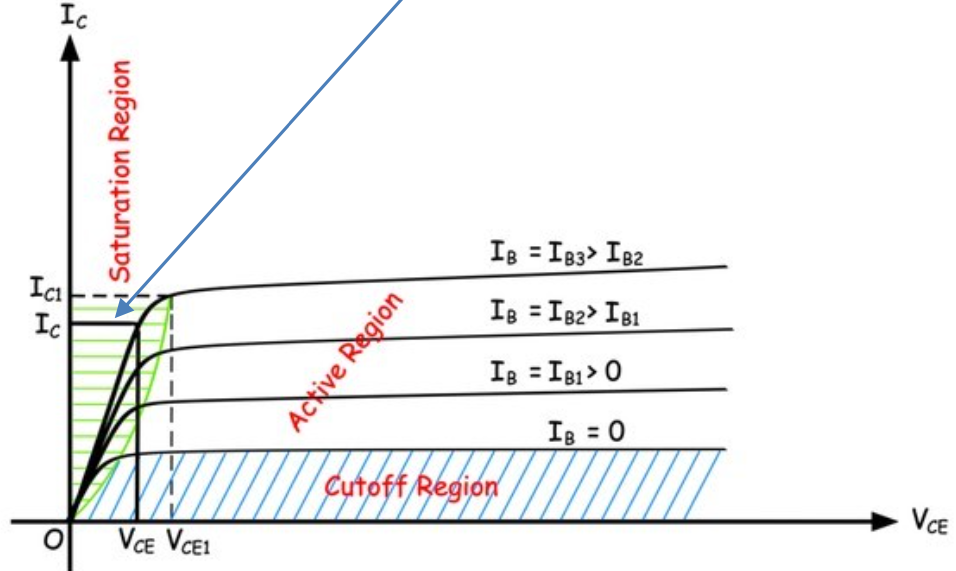
\includegraphics[scale=0.37,angle=0]{bjt_saturazione.png}
    \caption{Regione di saturazione}
    \label{saturazione}
\end{figure}

\subsection{Attiva inversa}
Nella regione attiva inversa la giunzione BC tra la base e il collettore è polarizzata \textit{direttamente}, mentre la giunzione BE tra la base e l'emettitore è polarizzata \textit{inversamente}. È sostanzialmente come nella regione attiva diretta ma con ruoli scambiati per il collettore e l'emettitore. Questo comporta che:
\begin{equation*}
    V_{be} < 0 \text{ \, \, } V_{ce} < V_{th}
\end{equation*}
Tuttavia in questa situazione si ha:
\begin{equation*}
    I_{e} \approx -\,I_{b}
\end{equation*}
cioè il guadagno in corrente del transistor è:
\begin{equation*}
    \frac{I_{e}}{I_{b}} \leq 1
\end{equation*}
questo perché il collettore \textit{non è bravo} come l'emettitore ad emettere elettroni e, viceversa, l'emettitore \textit{non è bravo} come il collettore a collezionare elettroni. 
\begin{figure}[h]
    \centering
    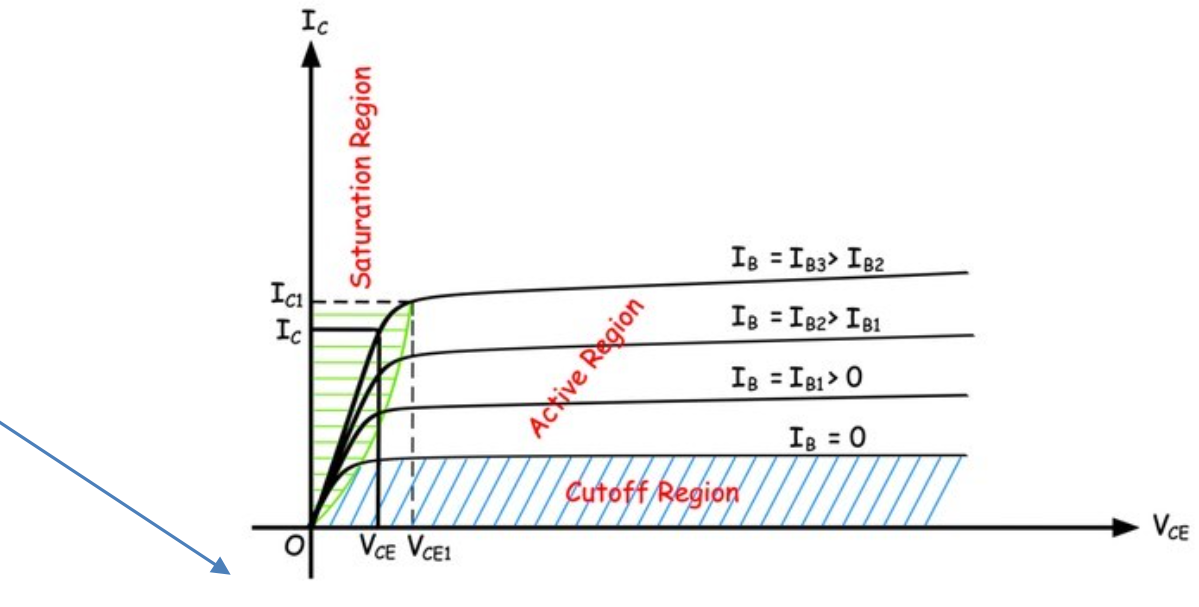
\includegraphics[scale=0.4,angle=0]{bjt_attiva_inversa.png}
    \caption{Regione attiva inversa}
\end{figure}

\section{Layout fisico}
Il BJT non è un dispositivo con una struttura simmetrica tra i tre terminali che lo compongono, ovvero non ha la struttura rappresentata in figura \ref{bjt}. In realtà, la sua realizzazione (effettuata su dei \textit{wafer}, sottili fette di materiale semiconduttore) prevede la creazione di sacche di drogante sia di tipo p che di tipo n.
\begin{figure}[h]
    \centering
    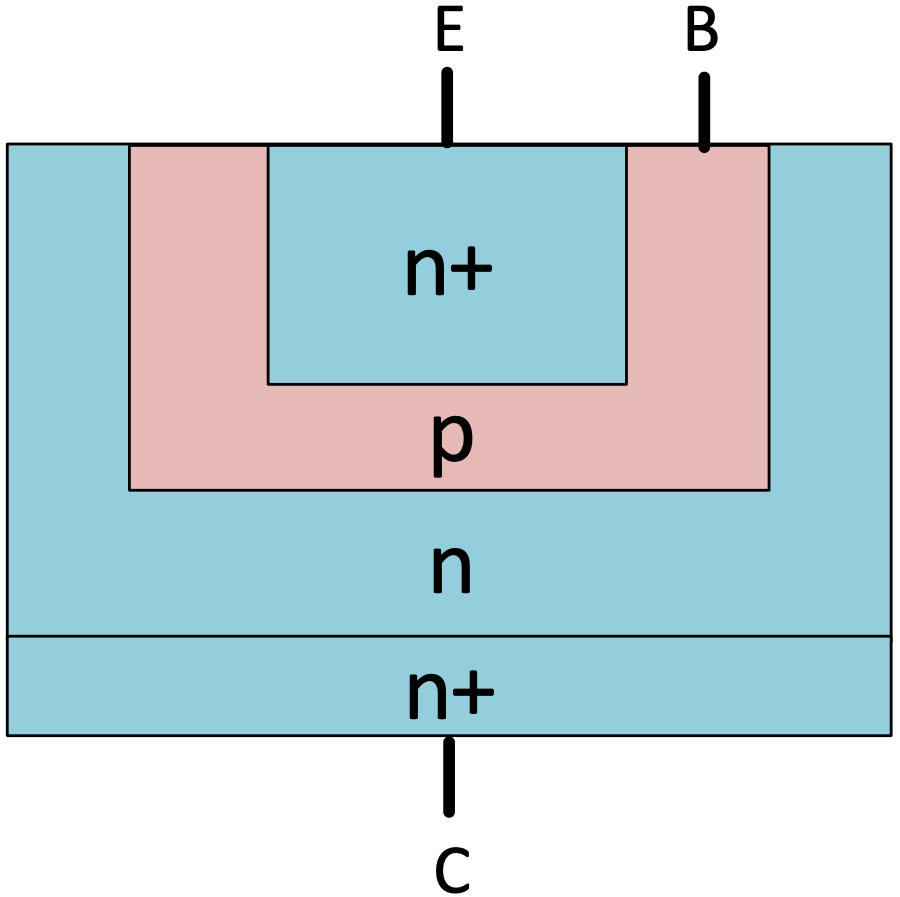
\includegraphics[scale=0.3,angle=0]{bjt_layout.png}
    \caption{Layout fisico di un BJT \textit{npn}}
\end{figure}
\\La regione n+ in basso serve semplicemente per la \textit{metallizzazione} del collettore. Il transistor vero e proprio è costituito da: l'emettitore (normalmente drogato \textbf{n+} dove il + sta a significare che è \textit{molto} drogato), la base (sottile, circonda l'emettitore, è drogata p) e il collettore (drogato n, circonda tutto l'emettitore). In questa configurazione l'emettitore, piccolo ma molto drogato, è facilmente generatore di elettroni e quando emette elettroni questi sono facilmente catturati dal collettore. Viceversa, se si polarizza in \text{attiva inversa} il dispositivo, il collettore può emettere elettroni ma, essendo un silicio drogato di tipo n e non n+, ne emette pochi e, per di più, ha una disposizione sfavorevole a causa della quale i pochi elettroni emessi hanno pochissima probabilità di essere catturati dall'emettitore mentre è molto più probabile che si ricombinino in base. È questo il motivo (asimmetria sia di drogaggio - n+ contro n - che di geometria) per cui il guadagno in regione attiva inversa è molto più piccolo del guadagno in regione attiva diretta.

\section{BJT pnp}
È il dispositivo perfettamente \textit{complementare} rispetto al BJT npn visto finora perché si ottiene scambiando i drogaggi: in questo transistor la base è drogata di tipo n mentre emettitore e collettore sono entrambi drogati di tipo p.
\begin{figure}[h]
    \centering
    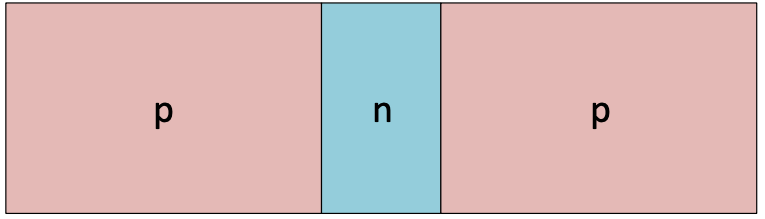
\includegraphics[scale=0.45,angle=0]{bjt_pnp.png}
    \caption{Struttura di un BJT di tipo \textit{pnp}}
\end{figure}

Nell'essere complementare al BJT npn si vanno a considerare le stesse equazioni del BJT pnp ma si usa una notazione di \textit{segno opposto} per le tre tensioni e correnti che caratterizzano il dispositivo.

Per le tensioni si considera \textit{positiva} la giunzione BE tra la base e l'emettitore quando il potenziale dell'emettitore è maggiore di quello della base ($V_{be} = V_{e} - V_{b}$ la freccia va dalla base all'emettitore), si considera \textit{positiva} la giunzione BC tra la base e il collettore quando il potenziale del collettore è maggiore di quella della base ($V_{bc} = V_{c} - V_{b}$ la freccia va dalla base al collettore), infine si considera \textit{positiva} la giunzione EC tra emettitore e collettore quando il potenziale dell'emettitore è maggiore di quello del collettore ($V_{ce} = V_{e} - V_{c}$ la freccia va dal collettore all'emettitore).

Per le correnti si considera \textit{positiva} la corrente entrante nell'emettitore e di conseguenza \textit{negative} le correnti uscenti dalla base e dal collettore.
\begin{figure}[h]
    \centering
    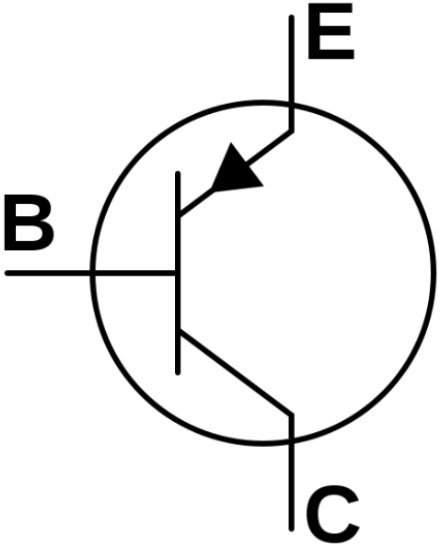
\includegraphics[scale=0.4,angle=0]{bjt_pnp_simbolo.png}
    \caption{Simbolo circuitale di un BJT \textit{pnp}}
\end{figure}

Le regioni operative sono le stesse del BJT npn: nella regione \textit{attiva diretta} la giunzione BE è polarizzata \textit{direttamente} cioè la tensione della base è più bassa di quella dell'emettitore e il collettore ha una tensione molto più bassa rispetto a base ed emettitore (infatti nel simbolo circuitale si dispongono i tre terminali per potenziale sempre più basso spostandosi dall'alto verso il basso - così la corrente andrà dall'alto verso il basso).

Nel BJT npn si parla di elettroni come portatori di carica, nel transistor pnp invece si parla di lacune che fungono da portatori di carica.

A livello statistico per definire il guadagno si deve tenere conto della \textbf{mobilità dei portatori}, ovvero quanto i portatori (che sono generati dall'emettitore) si muovono facilmente all'interno del materiale. Lacune ed elettroni non hanno la stessa mobilità, in particolare le lacune si muovono con una mobilità che è circa la \textit{metà} di quella con cui si muovono gli elettroni. Quindi dati due dispositivi geometricamente uguali ma con drogaggi tutti simmetricamente opposti, uno che sfrutta il moto degli elettroni come portatori di carica e l'altro che sfrutta il moto delle lacune, il dispositivo che sfrutta il moto delle lacune in genere sperimenta un guadagno in corrente che è circa la \textit{metà} di quello del dispositivo che sfrutta il modo degli elettroni. In questo caso, i transistor pnp hanno come portatori le lacune (essendo l'emettitore drogato p) che, muovendosi più lentamente, tendono più facilmente a ricombinarsi quando passano nella base e quindi il guadagno del dispositivo è minore rispetto a quello che si potrebbe ottenere con un transistor npn.\\

Riassumendo, per entrambi le tipologie di transistor bipolari si identificano quattro regioni operative:
\begin{description}
    \item[Cutoff] la giunzione base - emettitore è interdetta quindi non passa corrente né nella giunzione BE né in quella BC
    \item[Attiva diretta] la giunzione BE è polarizzata direttamente, quindi scorre corrente, mentre la giunzione BC è polarizzata inversamente. Il potenziale del collettore è molto elevato in valore assoluto e quindi il dispositivo si comporta come una sorgente di corrente controllata in corrente, dove il controllo è effettuato dalla corrente della base $I_{b}$, la sorgente di corrente è la corrente del collettore $I_{c}$ e il guadagno in corrente è $h_{fe}$
    \item[Saturazione] si ottiene abbassando progressivamente il valore assoluto del potenziale del collettore. Non c'è più possibilità di generare in modo costante tutta la corrente generata in regione attiva diretta, la corrente quindi diminuisce e la tensione può scendere fino ad un valore che generalmente è detta \textbf{tensione di saturazione} che vale $V_{ce-sat} \approx 0,2,\,V - 0,3\,V$. Il transistor non è più in grado di assorbire corrente
    \item[Attiva inversa] la giunzione BE è polarizzata inversamente e la giunzione BC è polarizzata direttamente. Si ottengono valori di guadagno di corrente molto bassi e minori o uguali di 1, passa poca corrente
\end{description}
\section{Fototransistor}
Un particolare dispositivo appartenente alla famiglia dei dispositivi optoelettronici insieme al fotodiodo è il \textbf{fototransistor}. Questo dispositivo è generalmente un transistor di tipo \textit{npn} con la particolarità che il terminale di base è \textit{assente}. Per polarizzare \textit{direttamente} la giunzione BE tra la base e l'emettitore si deve iniettare una \textbf{fotocorrente} invece di una corrente vera e propria. Per farlo vengono mandati dei fotoni sulla base del dispositivo e, una volta illuminata, per effetto dei fotoni vengono generate coppie elettrone-lacuna e queste coppie, se il collettore ha un potenziale sufficientemente elevato, generano una fotocorrente che scorre dalla base all'emettitore e che a sua volta si traduce in una molto maggiore corrente che scorre dal collettore all'emettitore. Questo significa che se $V_{c}$ è sufficientemente grande, il fototransistor è \textit{sempre} in regione \textit{attiva diretta}.
\begin{figure}[h]
    \centering
    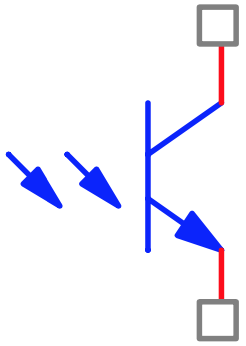
\includegraphics[scale=0.5,angle=0]{phototransistor.png}
    \caption{Simbolo circuitale di un fototransistor}
\end{figure}

Il vantaggio di questo dispositivo, che è sicuramente più complesso di un fotodiodo, è che si ha sempre un dispositivo a due terminali (come detto la base è assente) però la corrente che scorre in questo dispositivo è $h_{fe}$ volte la corrente che scorre nel relativo fotodiodo; il tutto a parità di luce incidente.

Viene utilizzato attaccando una resistenza al collettore (indicata con $R_{c}$) così da ottenere la tensione di polarizzazione del collettore $V_{cc}$, l'emettitore si mette a massa e la tensione di uscita $V_{out}$\, è quella del collettore. Sapendo che $I_{c} = h_{fe} \cdot I_{b}$ e che $I_{b}$ è proporzionale a $P_{in}$, la potenza luminosa in ingresso, si ottiene:
\begin{equation*}
    V_{out} = V_{cc} - ( R_{c} \cdot h_{fe} \cdot I_{b})
\end{equation*}
dove il termine $h_{fe} \cdot I_{b}$ viene visto come un unico termine, cioè $I_{c}$, che è ricavabile dal datasheet del fototransistor ed è generalmente centinaia di volte più grande dell'analogo per un fotodiodo. Oppure si può mettere la resistenza collegata non con il collettore ma con l'emettitore; in questo caso $V_{out}$ è la tensione dell'emettitore e vale $V_{out} =  R_{e} \cdot P_{in} \cdot G$ con \textit{G} il guadagno del fototransistor. Questi dispositivi si trovano all'interno dei telecomandi, dispositivi che in genere lavorano con gli infrarossi.

\chapter{MOS}
Il \textbf{MOS} è un dispositivo appartenente alla famiglia dei \textbf{FET}, ovvero dei \textit{transistors ad effetto di campo}, realizzato con tecnologia \textbf{metallo}, \textbf{ossido} e \textbf{semiconduttore}. Come per i BJT, anche per i MOS esistono due varianti: gli \textbf{N-MOS} e i \textbf{P-MOS}, rispettivamente a portatori elettroni e a portatori lacune. A differenza dei BJT che sono dispositivi controllati in corrente, i MOS sono dispositivi \textbf{controllati in tensione}. È per questo motivo che sono dei FET, perché è il campo elettrico che determina il funzionamento di questi dispositivi.

È un dispositivo a tre terminali, disposti come i tre terminali del transistor, e chiamati: \textbf{drain} (corrispondente al collettore del transistor), \textbf{gate} (corrispondente alla base) e \textbf{source} (corrispondente all'emettitore).

Le tensioni tra i tre terminali e le correnti sono definite nello stesso modo dei BJT. In particolare, i versi e i segni in un N-MOS sono definiti come nei BJT di tipo npn mentre in un P-MOS come in quelli di tipo pnp.

\section{N-MOS}
Un \textbf{N-MOS} è anche chiamato \textbf{mosfet a canale n}. È un dispositivo controllato in tensione nel senso che è la tensione di gate $V_{gs}$ a controllarne il funzionamento.
\begin{figure}[h]
    \centering
    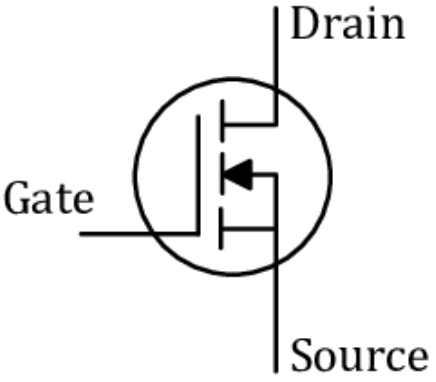
\includegraphics[scale=0.5,angle=0]{n_mos_simbolo.png}
    \caption{Simbolo circuitale di un N-MOS}
\end{figure}
\\Le tensioni sono definite come segue:
\begin{itemize}
    \item[$V_{sd}$]: la tensione tra drain e source. È \textit{positiva} quando drain è positivo rispetto a source, cioè quando $V_{d} > V_{s}$ perché $V_{ds}$ è la differenza tra il potenziale del drain $V_d$ e quello del source $V_s$
    \item[$V_{gs}$]: la tensione tra gate e source. È \textit{positiva} quando gate è positivo rispetto a source, cioè quando $V_{g} > V_{s}$
    \item[$V_{dg}$]: la tensione tra drain e gate. È \textit{positiva} quando gate è positivo rispetto a drain, cioè quando $V_{g} > V_{d}$
\end{itemize}
Analogamente le tre correnti, una per ognuno dei tre terminali del MOS, sono:
\begin{itemize}
    \item[$I_{d}$]: la corrente del drain, si prende \textit{positiva} quando è \textit{entrante} nel dispositivo
    \item[$I_{g}$]: la corrente del gate, si prende \textit{positiva} quando è \textit{entrante} nel dispositivo
    \item[$I_{s}$]: la corrente del source, si prende \textit{positiva} quando è \textit{uscente} dal dispositivo
\end{itemize}
La particolarità di un N-MOS è che la corrente del gate $I_{g}$ è \textit{sempre nulla} in tensione \textit{continua}. Questo aspetto è fondamentale per i dispositivi a basso consumo perché un dispositivo che consuma poco è un dispositivo nel quale, possibilmente, non ci sono correnti che scorrono continuamente. Tenere acceso un circuito logico composto da tanti transistors BJT necessita di polarizzare le loro basi con delle correnti (seppur minime), quindi consuma corrente. Al contrario, un circuito logico realizzato con dispositivi MOS ha la capacità di non consumare corrente quando non ci sono transizioni o di consumarne poca quando ce ne sono poche.
\begin{figure}[h]
    \centering
    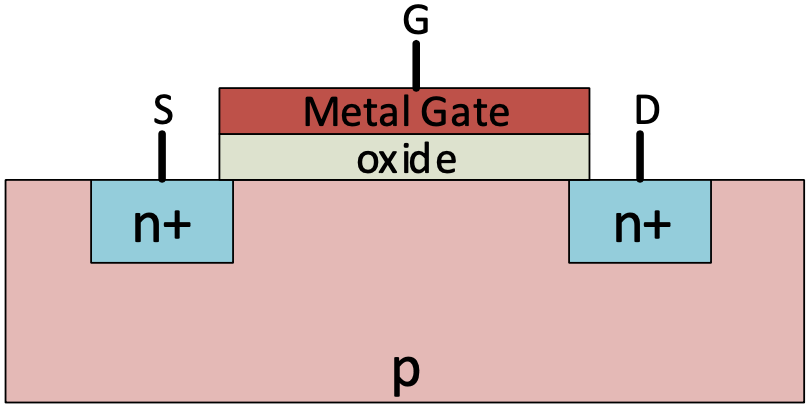
\includegraphics[scale=0.4,angle=0]{n_mos_struttura.png}
    \caption{Struttura di un N-MOS}
    \label{struttura_nmos}
\end{figure}
\\Un MOSFET a canale n è composto da una zona in silicio con drogaggio di tipo p sulla quale sono presenti due zone drogate n+ utilizzate per favorire la \textbf{metallizzazione} con l'esterno e in corrispondenza di queste due zone drogate n+ sono presenti i terminali source e drain.

La metallizzazione è necessaria perché gli scambi tra il dispositivo e l'esterno avvengono tramite i contatti esterni in alluminio e per far sì che avvenga la comunicazione tra dispositivo ed esterno si deve permettere di avere una giunzione che non sia \textit{raddrizzante}, ovvero che non sia una giunzione di tipo pn. Un materiale n+ (sopratutto se è molto n+), messo in contatto con l'alluminio che è un metallo, permette di creare una giunzione detta \textbf{ohmica} che non è raddrizzante.

È poi presente uno strato di \textbf{ossido} di dimensioni molto limitate (frazioni del micron) che viene utilizzato nell'industria dei semiconduttori come materiale \textit{isolante} e viene generalmente realizzato in \textit{biossido di silicio} oppure in \textit{nitruro di silicio}, entrambi forme vetrose del silicio altamente isolanti. Quindi questo strato di ossido ha un aspetto vetroso e una rigidità dielettrica, cioè un potere isolante, come quella del vetro (molto isolante). Su questo strato di ossido è poggiato un metallo che costituite il terzo terminale: il gate.

La sequenza di materiali: semiconduttore di tipo p, ossido e metallo definisce proprio la struttura MOS caratteristica di questi dispositivi.

Dal gate in metallo al semiconduttore di tipo p \textit{non} può scorrere corrente perché tra di loro è presente lo strato di ossido isolante. È questo il motivo per cui, in condizione di tensione continua, la corrente del gate è sempre nulla: perché non scorre corrente continua dal gate alla zona p. 

Tuttavia, questa struttura è a sua volta una struttura di materiali conduttori separati da un isolante a facce piane e parallele (nello specifico un conduttore e un semiconduttore paralleli e separati da uno strato isolante), cioè è un \textbf{condensatore} e questo comporta che, variando la tensione ai capi del condensatore o passando in tensione \textit{alternata}, ci saranno delle cariche che scorreranno, ovvero sui transitori ci sarà effettivamente della corrente che servirà per caricare e scaricare la \textit{capacità equivalente} del gate.

\section{Funzionamento}
Per costruzione, in condizioni stazionarie tra source e drain non può passare corrente perché i due terminali sono collegati tramite due giunzioni pn simmetriche disposte come in un BJT di tipo npn, cioè due diodi opposti uno dei quali è sempre polarizzato inversamente. Rispetto alla struttura transistor, la zona p, chiamata \textbf{canale}, non è stretta e questo comporta che la separazione tra le due zone n è molto pronunciata.

Un N-MOS inizia a funzionare nel momento in cui si va ad applicare una tensione di gate \textit{positiva} cioè $V_{gs} > 0$ rispetto al resto del circuito (in particolare rispetto al materiale di tipo p). Ciò che succede quando si applica una tensione positiva al gate è esattamente che succede all'interno di un condensatore: sulla piastra soggetta al potenziale positivo, corrispondente al gate, si accumulano le cariche positive, mentre sulla piastra opposta, la porzione del semiconduttore di tipo p a contatto con lo strato di ossido, vengono attratte cariche negative. Queste cariche negative accumulate vanno ad occupare gli spazi disponibili delle lacune che quindi vengono riempite con portatori di elettroni (come succedeva nella giunzione pn) e si crea una \textbf{regione di svuotamento}.
\begin{figure}[h]
    \centering
    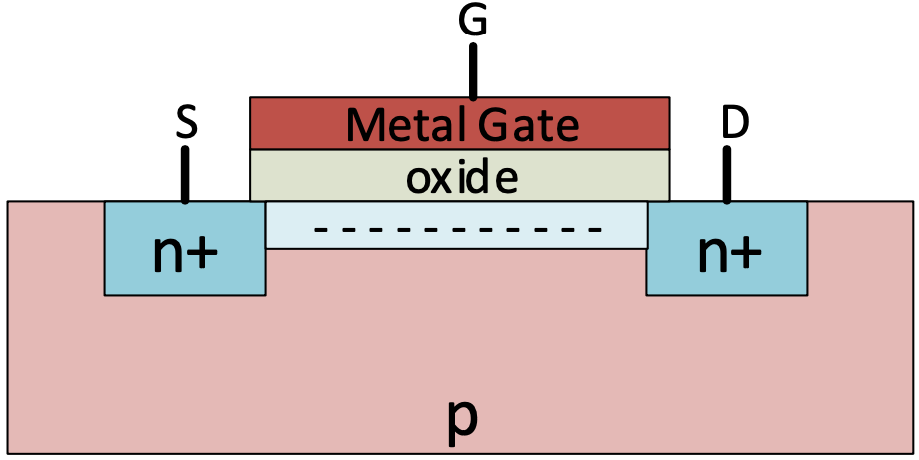
\includegraphics[scale=0.4,angle=0]{n_mos_svuotamento.png}
    \caption{Accumulo della cariche negative}
\end{figure}
\\Essendosi creata un regione di svuotamento, le cariche sono tutte bloccate dentro le lacune libere e questo comporta che non si possano avere fenomeni di scorrimento di cariche: ci si trova ancora in una situazione di stazionarietà.

Continuando ad aumentare la tensione di gate $V_{gs}$, questa finirà per superare un certo valore di soglia $V_t$. Quando $V_{gs} > V_t$ il campo elettrico che si forma all'interno del condensatore è così elevato che riesce a tirare ulteriori elettroni prendendoli dalle due zone a drogaggio n+ e portandoli nella zona p nella quale si erano già accumulate delle cariche negative.
\begin{figure}[h]
    \centering
    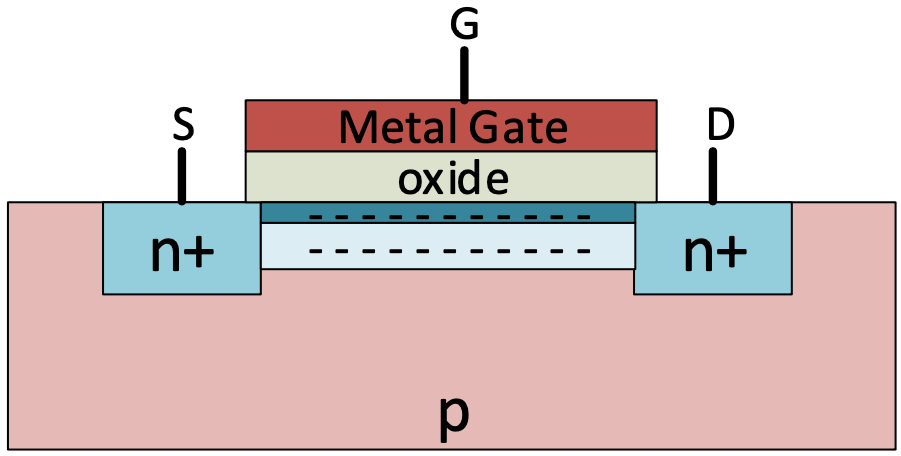
\includegraphics[scale=0.4,angle=0]{n_mos_canale.png}
    \caption{Accumulo della cariche negative}
    \label{svuotamento}
\end{figure}
\\Questi ulteriori elettroni (provenienti sopratutto dal source perché si sta applicando una differenza di potenziale $V_{gs} = V_{g} - V_s$ tra gate e source per utilizzare il source come connessione al terzo terminale: il drain) sono tutti elettroni \textit{liberi}, cioè sono elettroni in eccesso rispetto a quelli che avevo riempito il reticolo cristallino inserendosi nelle lacune per creare la regione di svuotamento e si vanno a disporre al di sotto del gate. A questo punto si è creato un \textbf{canale conduttivo } di elettroni tra source e drain, cioè una zona che sarebbe l'equivalente di una zona drogata n+ perché ha un eccesso notevole di elettroni. Se ora si va ad applicare un potenziale al drain, il canale conduttivo che si è creato permette lo scorrimento di corrente tra source e drain. Tanto maggiore è la tensione $V_{gs}$ tra gate e source, tanti più elettroni saranno disponibili nel canale conduttivo e tanto migliore la sarà la conduzione tra source e drain.

\section{Regioni operative}
Il dispositivo N-MOS è caratterizzato da tre possibili regioni di funzionamento: la regione di \textbf{cutoff}, la regione \textbf{lineare} e la regione di \textbf{saturazione}.

\subsection{Cutoff}
Nella regione di cutoff o \textbf{di interdizione} la tensione tra gate e source non ha ancora raggiunto la tensione di soglia:
\begin{equation*}
    V_{gs} < V_{t}
\end{equation*}
In questa situazione non ci sono portatori di elettroni nel canale e questo comporta che \textit{non} c'è conduzione tra drain e source.

Per tensioni $V_{gs}$ molto basse, minori della tensione di soglia $V_{t} = 2\,V$, il dispositivo sta lavorando in una regione in cui la corrente di drain $I_{d}$ è \textit{nulla}, come si vede nel grafico di sinistra. Non passa corrente tra drain e source, il che significa che il dispositivo è spento.
\begin{figure}[h]
    \centering
    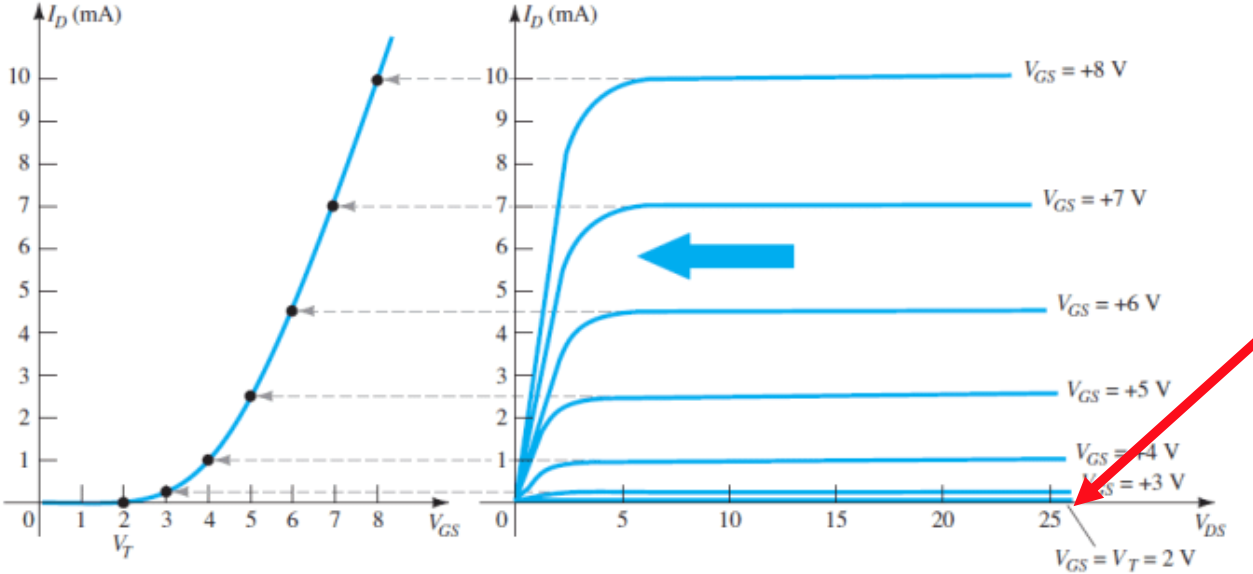
\includegraphics[scale=0.42,angle=0]{n_mos_cutoff.png}
    \caption{Regione di cutoff}
\end{figure}
\\Il grafico di destra ha la tensione $V_{ds}$ sull'asse \textit{x} e la corrente di drain $I_{d}$ sull'asse \textit{y} (in condizione statica è anche la corrente di source $I_{s}$). Nel grafico di sinistra invece, è rappresentato l'andamento della tensione di saturazione $I_{d-sat}$ rispetto alla tensione tra gate e source $V_{gs}$.

\subsection{Lineare}
Nella regione lineare il dispositivo MOS inizia a condurre perché la tensione del gate supera la tensione di soglia:
\begin{equation*}
    V_{gs} > V_{t}
\end{equation*}
Per ogni tensione di gate si identifica una specifica curva nel grafico di destra. Tutte le curve tendono a salire seguendo un andamento simile; in particolare: più alta è la tensione di gate e più la curva è ripida e alta. Con correnti di drain ragionevolmente basse, cioè
\begin{equation*}
    I_{d} < I_{d-sat}
\end{equation*}
ci si trova a lavorare in una regione prossima all'asse \textit{y} con tensioni $V_{gs}$ comprese tra $0\,V$ e circa $5\,V$. In questa regione il dispositivo ha un andamento \textit{lineare} con un comportamento che ricorda quello di una \textit{resistenza}; ovvero la corrente $I_{d}$ è \textit{direttamente proporzionale} alla tensione $V_{ds}$ con costante di proporzionalità chiamata \textbf{resistenza di canale} il cui valore è specificato all'interno del datasheet del dispositivo MOS. Ovviamente, la resistenza di canale è inversamente proporzionale, secondo una qualche legge, alla tensione di gate. Non a caso, a valori alti di $V_{gs}$ corrispondono curve più rapide che rappresentano resistenza basse.

Superato un certo valore massimo di corrente $I_{d-sat}$, le curve tendono a diventare parallele all'asse x fermandosi su certo valore per la corrente di drain $I_{d}$.
\begin{figure}[h]
    \centering
    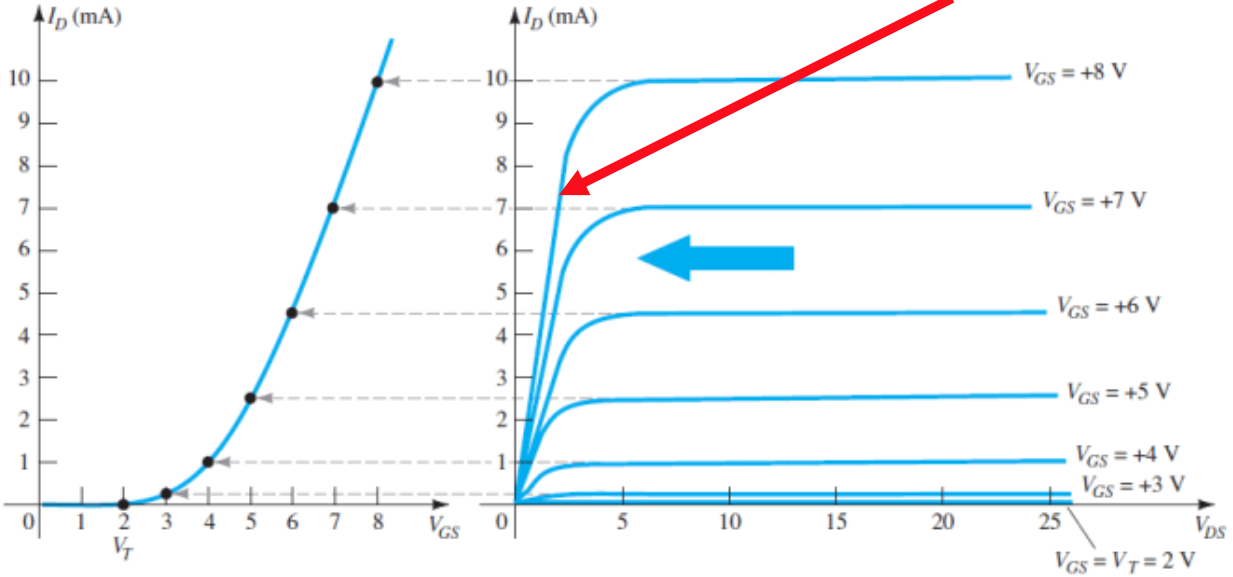
\includegraphics[scale=0.42,angle=0]{n_mos_lineare.png}
    \caption{Regione lineare}
\end{figure}

\subsection{Saturazione}
Questa situazione si verifica nel momento in cui la tensione di gate $V_{gs}$ ha superato la tensione di soglia e, per un qualsiasi valore della tensione di drain $V_{ds}$ maggiore di un certo valore, la corrente di drain $I_{d}$ non aumenta più ma si ferma al valore di saturazione $I_{d-sat}$.

Di fatto, il dispositivo si comporta come un \textbf{generatore costante di corrente comandato in tensione}; dalla tensione di gate $V_{gs}$. Maggiore è la tensione di gate e maggiore è la corrente di saturazione.
\begin{figure}[h]
    \centering
    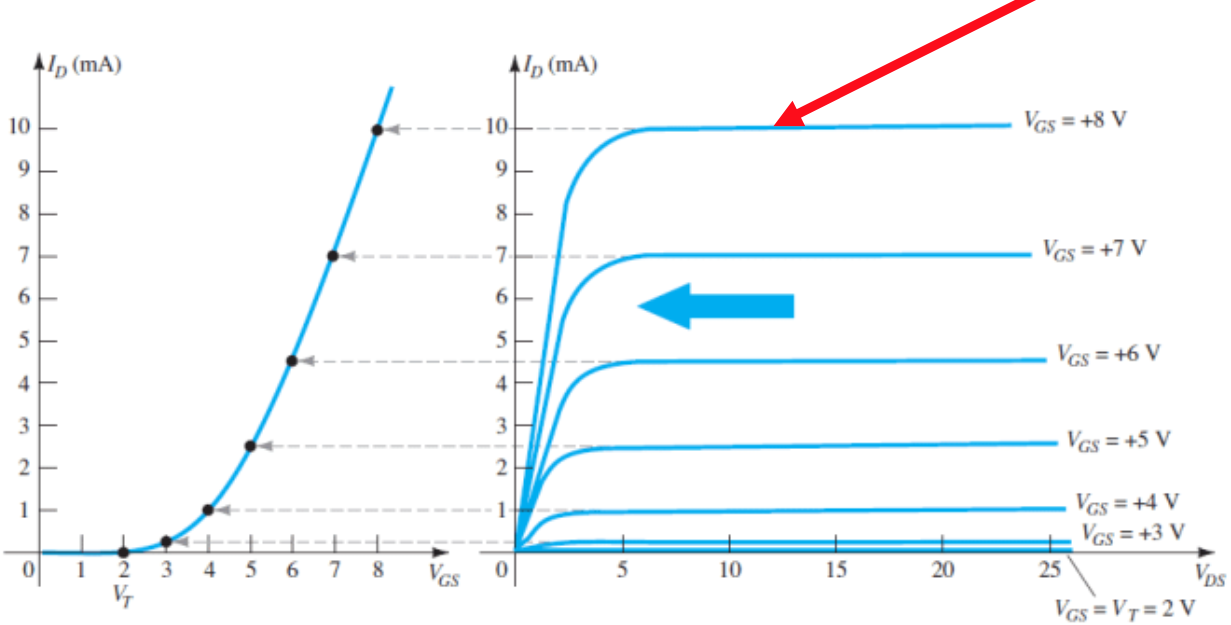
\includegraphics[scale=0.4,angle=0]{n_mos_saturazione.png}
    \caption{Regione di saturazione}
\end{figure}
\subsection{Confronto con il BJT}
La regione di saturazione del BJT è quella regione che corrisponde alla regione lineare di un MOS. Al contrario, la regione attiva diretta (anche chiamata regione lineare) del BJT corrisponde alla regione di saturazione del MOS. Nel caso del MOSFET si parla di saturazione in riferimento alla sua capacità di far passare corrente: sfruttando la tensione di gate $V_{gs}$ sono stati inseriti un certo numero di portatori ma se la differenza di potenziale $V_{ds}$ viene aumentata molto i portatori vengono tutti strappati dal canale che di fatto viene chiuso perché gli vengono tolti gli elettroni di conduzione. Il drain ha tensione positiva che può essere maggiore della tensione di gate, quindi lavora nel verso opposto a come lavora il source cioè, data una certa tensione $V_{gs}$ il source immette elettroni di conduzione mentre il drain, che è a tensione positiva, li toglie quando la sua tensione è maggiore di zero.

\section{Corrente}
Esiste una relazione ben precisa tra le tensioni di gate e drain e la corrente di drain che è definita tramite un'equazione di secondo grado chiamata \textbf{equazione del MOSFET}:
\begin{equation}
    I_{d} = K\,[2(V_{gs} - V_{t})V_{ds} - V_{ds}^2]
\end{equation}
È una \textit{parabola} in $V_{ds}$ con concavità rivolta verso il basso e con coefficiente lineare $2K(V_{gs} - V_{t})$ legato alla tensione di gate. Questa equazione è valida per $V_{gs} > V_{t}$, corrispondente alla regione lineare del dispositivo, e solo fino al \textit{vertice} della parabola che corrisponde al valore massimo di $I_{d}$, cioè al valore di saturazione $I_{d-sat}$. Non a caso se $V_{gs} < V_{t}$ ci si trova nella regione di cutoff del MOS in cui la corrente di drain è nulla e il dispositivo è spento. Il valore di saturazione è definito come:
\begin{equation}
    I_{d-sat} = K(V_{gs} - V_{t})^2
    \label{id_sat}
\end{equation}
che, come si nota nel grafico di sinistra nelle tre foto precedenti, ha un andamento \textit{parabolico} a partire dalla tensione di soglia $V_t$ mentre è \textit{nulla} per $V_{gs} < V_{t}$. L'ascissa del vertice della parabola corrisponde al punto in cui $V_{ds} = V_{gs} - V_{t}$. Dunque nel grafico che ha per ordinata la corrente di drain $I_{d}$ (quello a destra) il vertice della parabola ha ascissa $V_{ds} + V_{t}$ e coordinata $K(V_{gs} - V_{t})^2$.

Per tutte le tensioni $V_{ds} \geq V_{gs} - V_{t}$ ci si trova in saturazione: la corrente $I_{d}$ è costante identicamente pari alla corrente di saturazione $I_{d-sat}$ definita tramite la \eqref{id_sat}. Riassumendo:
\begin{equation*}
I_{d} = \left\{
\begin{array}{ll}
0 &\text{se } V_{gs} < V_{t}\\
K\,[2(V_{gs} - V_{t})V_{ds} - V_{ds}^2] &\text{se } V_{gs} > V_{t} \text{ e } V_{gs} < V_{ds} + V_{t}\\
K(V_{gs} - V_{t})^2 & \text{se } V_{ds} \geq V_{gs} - V_{t} 
\end{array}\right.
\end{equation*}
L'andamento di $I_{d}$ è esattamente quello rappresentato dalle curve nel grafico di destra nelle tre figure precedenti. Questi grafici sono disponibili all'interno del datasheet del dispositivo.

Queste curve variano al variare del parametro $V_{gs} - V_{t}$ che di fatto controlla il valore massimo di corrente che si può raggiungere e il punto in cui è possibile raggiungerlo. È questo il motivo per cui si dice che un N-MOS è un dispositivo controllato in tensione: perché il suo funzionamento è dettato dal parametro $V_{gs} - V_{t}$ che funge da variabile di controllo tramite la quale è possibile definire la corrente $I_{d}$ al variare della tensione $V_{ds}$.

La costante \textit{K} è definita secondo l'equazione:
\begin{equation}
    K = \frac{1}{2}\mu C_{ox}\frac{W}{L}
\end{equation}
Dipende dalla mobilità dei portatori $\mu$ e dai parametri geometrici del dispositivo \textit{W} e \textit{L} che sono rispettivamente la larghezza e la lunghezza del canale, entrambe controllate dal gate.
È \textit{direttamente proporzionale} alla mobilità dei portatori $\mu$ che, nel caso di un N-MOS, corrisponde alla mobilità degli elettroni mentre in un P-MOS corrisponde a quella delle lacune.
Per definizione, tanto più largo è il canale e tanto maggiore sarà \textit{K}, cioè tanto maggiore sarà la corrente che potrà passare nel canale. Viceversa, tanto più lungo è il canale e tanto minore sarà \textit{K} perché i portatori dovranno spostarsi per un tratto più lungo impiegando quindi uno sforzo maggiore (il canale può essere visto come una resistenza). A parità di condizioni, confrontando il K di un MOS a canale n e di uno a canale p, si ha che: \begin{equation*}
    K_{b} \approx 2K_{p}
\end{equation*}

\section{P-MOS}
Anche chiamato \textbf{mosfet a canale p}, è il dispositivo \textit{complementare} ad un N-MOS. Il canale di un P-MOS sarà quindi caratterizzato da lacune e non più da elettroni. Dal punto di vista circuitale è analogo ala transistor di tipo \textit{pnp}.
\begin{figure}[h]
    \centering
    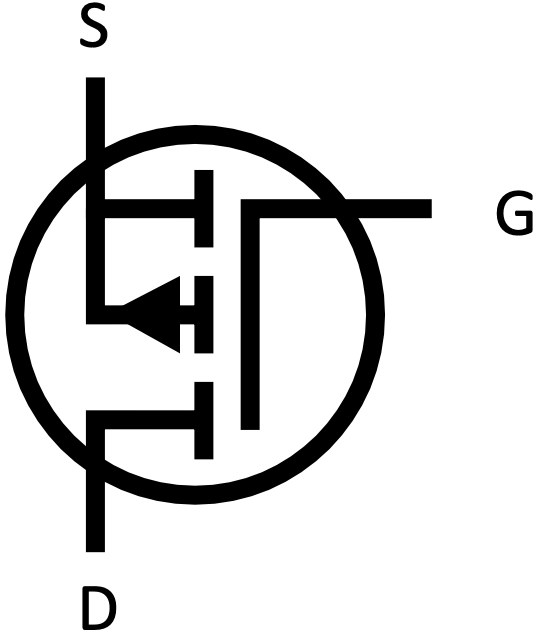
\includegraphics[scale=0.35,angle=0]{p_mos_simbolo.png}
    \caption{Simbolo circuitale del P-MOS}
\end{figure}
\\Per quanto riguarda le tensioni:
\begin{itemize}
    \item[$V_{sd}$]: la tensione tra drain e source. Il source si suppone essere sempre \textit{positivo} mentre il drain si suppone essere sicuramente \textit{negativo} rispetto al source
    \item[$V_{gs}$]: la tensione tra gate e source. Il gate è \textit{negativo} rispetto al source
    \item[$V_{dg}$]: la tensione tra drain e gate
\end{itemize}
Le tre correnti sono così definite:
\begin{itemize}
    \item[$I_{s}$]: la corrente del source, si prende \textit{positiva} quando è \textit{entrante} nel dispositivo
    \item[$I_{d}$]: la corrente del drain, si prende \textit{positiva} quando è \textit{uscente} dal dispositivo
    \item[$I_{g}$]: la corrente del gate
\end{itemize}
Applicando inizialmente una tensione di gate $V_{gs}$ (negativa per definizione) minore, cioè \textit{più negativa}, di una tensione di soglia negativa $V_{gs} < - |V_{t}|$, si crea una \textbf{regione di svuotamento} (come in figura \ref{svuotamento}) del tutto complementare a quella che si forma all'interno di un N-MOS. Questa complementarietà è dovuta al fatto che dentro un P-MOS è presente una vasta zona in silicio drogato di tipo n sulla quale sono presenti due piccole zone drogate p+ in corrispondenza di source e drain. La zona a drogaggio n è poi in contatto con uno strato di ossido isolante sopra il quale è collocato il gate in metallo. La presenza della zona drogata n (e non p come in un N-MOS) comporta che dentro di essa, in corrispondenza della regione di svuotamento, si vanno ad accumulare delle lacune che formano una carica positiva nel semiconduttore mentre se ne crea una negativa nel gate.
\begin{figure}[h]
    \centering
    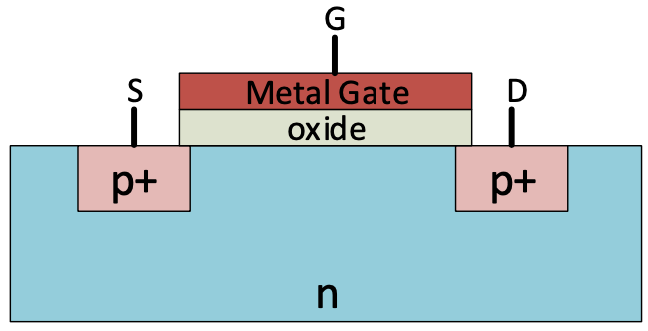
\includegraphics[scale=0.45,angle=0]{p_mos_struttura.png}
    \caption{Struttura di un P-MOS}
\end{figure}

Diminuendo ancora di più la tensione di gate, quando sarà sufficientemente negativa sarà in grado di attrarre ulteriori lacune dalle due zone p+ adiacenti, queste lacune si disporranno al di sotto della regione di svuotamento e, essendo lacune libere, potranno fungere da portatori di carica. Potrà quindi scorrere corrente tra i terminali drain e source. Tuttavia in questa corrente saranno le lacune a muoversi ma esse hanno una mobilità che è circa la metà di quella degli elettroni (come già detto parlando dei BJT) e questo fa sì che le prestazioni di un P-MOS siano generalmente \textit{minori} rispetto a quelle di un N-MOS. A parità di funzionamento, il P-MOS porta metà corrente rispetto a quella portata da un N-MOS.\\

Riassumendo, per entrambi le tipologie di MOSFET, si quella a canale n che quella a canale p, si identificano tre regioni operative:
\begin{description}
    \item[Cutoff] non c'è conduzione tra source e drain perché $|V_{gs}| < |V_{t}|$ implica che non può scorrere corrente all'interno del canale
    \item[Regione lineare] in questo caso $|V_{gs}| > |V_{t}|$ e $|I_{d}| < |I_{d-sat}|$. Finché non si raggiunge la corrente limite $I_{d-sat}$ dettata dalla tensione $V_{gs}$, si ha un andamento inizialmente lineare e poi più marcatamente parabolico della corrente. In queste condizioni il dispositivo si comporta come un resistore controllato in tensione
    \item[Saturazione] in questo caso $|I_{d}| = |I_{d-sat}|$. Si è raggiunto il valore limite della corrente definito tramite l'equazione \eqref{id_sat}. La corrente non cresce più, quindi l'uscita è costante indipendentemente dalla tensione applicata sul drain. In queste condizioni il dispositivo si comporta come un generatore di corrente costante controllato in tensione
\end{description}

\section{N-MOS reale}
Nella realtà fisica, un dispositivo N-MOS è \textbf{asimmetrico} per costruzione. In particolare, la metallizzazione del source tramite l'impiego dell'alluminio mette in \textit{cortocircuito} anche una parte del semiconduttore drogato p, quindi il source e il \textbf{body} del diodo sono collegati insieme: una certa zona del semiconduttore di tipo p (la parte bassa della zona p riportata in figura \ref{struttura_nmos}) ha lo stesso potenziale del source. Questo comporta che si viene a creare un diodo, chiamato \textbf{body diode}, tra il drain e il source messo in cortocircuito con il semiconduttore di tipo p. Questo diodo è presente nella maggior parte dei MOSFET. È questo il motivo per cui, in condizioni normali, per avere il comportamento finora descritto, si deve avere il potenziale di drain \textit{maggiore} di quello di source perché se così non fosse il diodo body si polarizzerebbe \textit{direttamente} e scorrerebbe corrente dal source al drain senza nessun controllo da parte del gate, cioè indipendentemente dalla tensione di gate.
\begin{figure}[h]
    \centering
    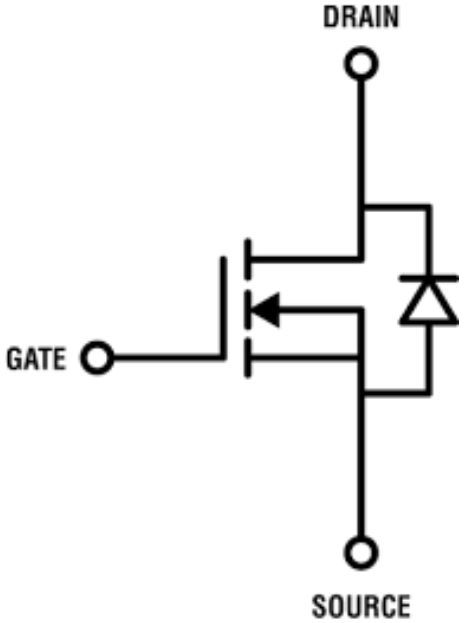
\includegraphics[scale=0.4,angle=0]{n_mos_reale.png}
    \caption{Body diode}
\end{figure}
\\Al contrario, in un MOS a canale p si deve fare in modo che il drain sia sempre più \textit{negativo} del source.

Indipendentemente dalla tipologia di MOS, come nel caso dei diodi e transistor, ci sono delle limitazioni riguardo le tensioni che possono essere applicate al drain e se queste non sono rispettate il dispositivo si romperà. Questo perché se la tensione applicata al drain è troppo elevata (maggiore della \textbf{tensione di breakdown}), il campo elettrico che si crea tra drain e source è così elevato da perforare il canale. In questo scenario le curve di corrente $I_{d}$ impennano rapidamente verso l'alto e questo di fatto rappresenta la rottura del dispositivo.

\section{Impiego dei MOS}
Normalmente si utilizzano sia i P-MOS che gli N-MOS. Nelle logiche C-MOS sono presenti le due tipologie accompagnate da alcuni accorgimenti per garantire che entrambe abbiano la stessa prestazione. Nell'elettronica di potenza, in cui si utilizzano questi dispositivi come interruttori o per svolgere compiti gravosi in termini di potenza richiesta, si cerca di sfruttare al meglio gli N-MOS grazie alle loro prestazioni nettamente migliori in modo del tutto analogo al contesto dei BJT in cui si tendono a preferire quelli di tipo npn. 
\begin{figure}[h]
    \centering
    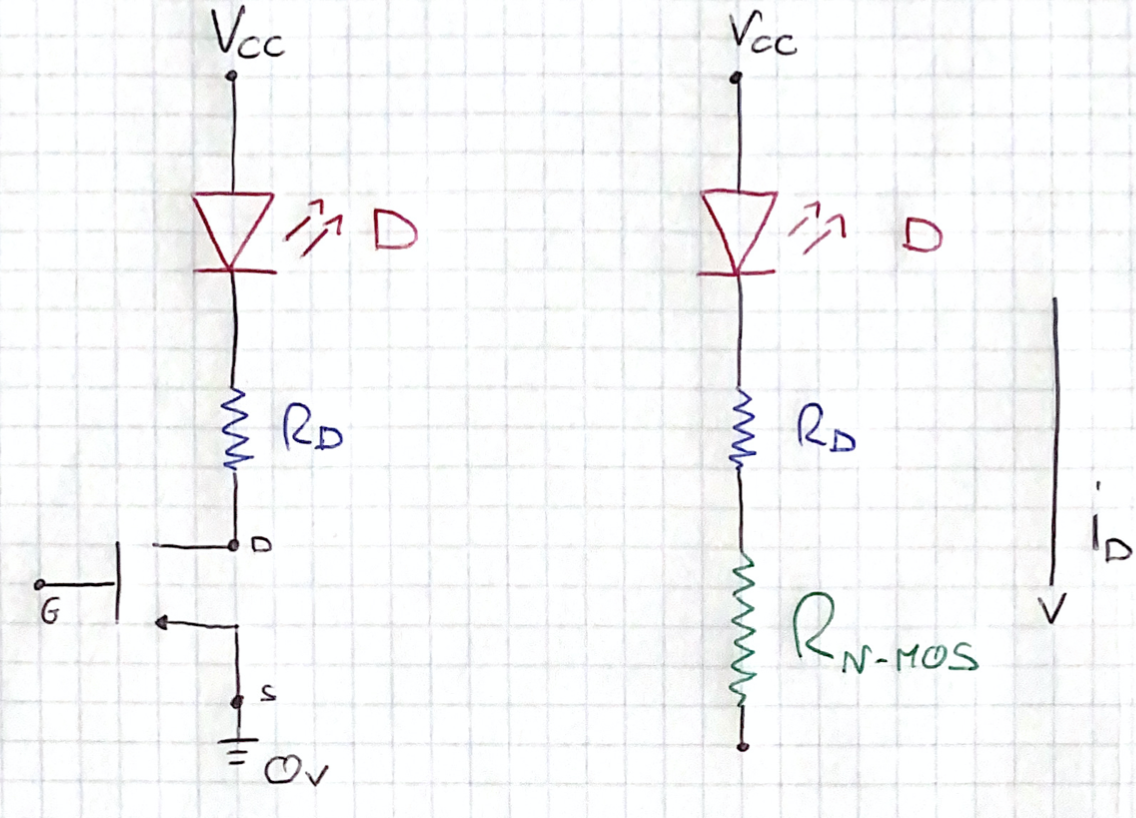
\includegraphics[scale=0.35,angle=0]{mos_interruttore.png}
    \caption{Body diode}
\end{figure}
\\Nel seguente circuito, il MOS a canale n viene utilizzato come interruttore per gestire il carico soggetto ad una tensione $V_{cc}$ e composto da una resistenza $R_{d}$ e da un LED $D$ da accendere. Il carico è collegato al drain, il source viene messo a $0\,V$ mentre il gain riceve un segnale in ingresso. Quando la tensione applicata sul gate è maggiore della tensione di soglia $V_{t}$, si attiverà il canale del gate tra source e drain trasformandolo in una opportuna resistenza. Se per esempio il gate è soggetto ad una tensione di $5\,V$ e la tensione di soglia del MOS è $V_{t} = 2\,V$, si può sostituire il MOS con la corrispettiva \textit{resistenza di canale} $R_{n-mos}$ il cui valore è fornito dal datasheet del dispositivo. A questo punto si deve determinare la corrente che scorre nel circuito e poi controllare che valga $I_{d} < I_{d-sat}$, se è vero significa che il MOS si sta effettivamente comportando come una resistenza, come se fosse un interruttore. Se invece $I_{d} > I_{d-sat}$, l'ipotesi di resistenza di canale decade e la corrente sarà limitata alla corrente di saturazione $I_{d} = I_{d-sat}$.

\chapter{Circuiti logici digitali}
I \textbf{circuiti logici digitali} sono tutti quei circuiti in cui l'informazione è \textbf{quantizzata} in soli due possibili livelli chiamati \textbf{stati digitali}: alto e basso, vero o falso, 0 o 1. Alla base di tutto c'è l'\textbf{algebra di Boole}, l'aritmetica binaria. L'impiego di solo due livelli possibili permette di semplificare il trasferimento dell'informazione da un dispositivo all'altro perché il ricevente è in grado di discriminare facilmente i due stati.

\section{Operatori booleani}
Per poter effettuare delle operazioni logiche si sfrutta l'algebra booleana tramite la quale si definiscono gli \textbf{operatori booleani}.
\begin{itemize}
    \item\textbf{AND}: indicato con una linea sopra l'operando che deve essere negato.
    \begin{figure}[h]
    \centering
    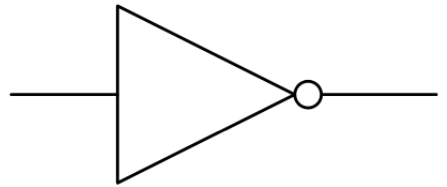
\includegraphics[scale=0.5,angle=0]{logica_not.png}
    \caption{Simbolo circuitale del NOT}
    \end{figure}
    \\La sua tabella di verità è la seguente:
    \begin{table}[h]
        \centering
        \begin{tabular}{c|c}
        \em A & $\overline{A}$\\\hline
        0 &1\\
        1 &0
        \end{tabular}
        \caption{Tabella di verità del NOT}
    \end{table}
    \item\textbf{AND}: indicato come il prodotto tra i due operandi, è la moltiplicazione binaria.
    \begin{figure}[h]
        \centering
        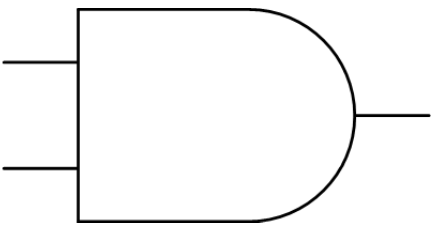
\includegraphics[scale=0.5,angle=0]{logica_and.png}
        \caption{Simbolo circuitale dell'AND}
    \end{figure}
    \\L'uscita dell'AND è vera solo se tutti gli ingressi sono veri. La sua tabella di verità è:
    \begin{table}[ht]
        \centering
        \begin{tabular}{c c |c}
        \em A &\em B &$A \cdot B$\\\hline
        0 &0 &0\\
        0 &1 &0\\
        1 &0 &0\\
        1 &1 &1
        \end{tabular}
        \caption{Tabella di verità dell' AND}
    \end{table}
    \item\textbf{OR}: indicato come la somma tra i due operandi, è la somma logica.
    \begin{figure}[h]
        \centering
        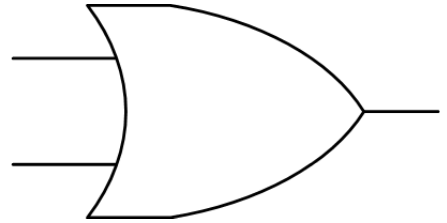
\includegraphics[scale=0.5,angle=0]{logica_or.png}
        \caption{Simbolo circuitale dell' OR}
    \end{figure}
    \\L'uscita dell'AND è vera se almeno uno degli ingressi è vero. La sua tabella di verità è la seguente:
    \begin{table}[h]
        \centering
        \begin{tabular}{c c |c}
        \em A &\em B &$A + B$\\\hline
        0 &0 &0\\
        0 &1 &1\\
        1 &0 &1\\
        1 &1 &1
        \end{tabular}
        \caption{Tabella di verità dell' OR}
    \end{table}
\end{itemize}
\subsection{Leggi di De Morgan}
Le \textbf{leggi di De Morgan} sono leggi relative alla logica booleana utilizzate per l'analisi di circuiti logici e stabiliscono relazioni di equivalenza tra gli operatori logici AND e OR. I due teoremi sono duali tra loro:
\begin{itemize}
    \item Riscrivendo l'operazione di disgiunzione logica come
    \begin{equation*}
        A + B = \overline{\overline{A} \cdot \overline{B}}
    \end{equation*}
    si ricava la prima legge di De Morgan secondo la quale:
    \begin{equation}
        \overline{A + B} = \overline{A} \cdot \overline{B}
    \end{equation}
    dove $\overline{A + B}$ è la negazione dell'operazione logica OR che viene chiamata \textbf{NOR}.
    \item Considerando la congiunzione logica come
    \begin{equation*}
        A \cdot B = \overline{\overline{A} + \overline{B}}
    \end{equation*}
    si ricava la seconda legge di De Morgan, duale alle prima:
    \begin{equation}
        \overline{A \cdot B} = \overline{A} + \overline{B}
    \end{equation}
    con $\overline{A \cdot B}$ la negazione logica dell'AND chiamata \textbf{NAND}.
\end{itemize}

\subsection{Universalità}
Utilizzando i tre operatori logici AND, OR e NOT è possibile descrivere tutte le funzioni logiche per un qualsiasi numero di ingressi e uscite. Questo perché tramite la formule di De Morgan si può passare da una forma logica di somma ad una di prodotto e viceversa e questo permette di scambiare tra di loro le porte logiche. Una qualsiasi funzione booleana può essere espressa come prodotto di somme o come somma di prodotti e negazioni.

In particolare, per sintetizzare una qualsiasi funzione logica ci sono essenzialmente tre possibili gruppi di porte logiche da utilizzare:
\begin{enumerate}
    \item La porta NOT e almeno una porta tra AND, OR, NAND e NOR
    \item La sola porta NOR questo perché mettendo in cortocircuito i due terminali di ingresso alla porta si ottiene una porta NOT
    \item La sola porta NAND per lo stesso motivo detto sopra
\end{enumerate}
Se per esempio si considera la porta NOR, la sua tabella di verità è la seguente:
\begin{table}[ht]
        \centering
        \begin{tabular}{c c |c}
        \em A &\em B &$\overline{A + B}$\\\hline
        0 &0 &1\\
        0 &1 &0\\
        1 &0 &0\\
        1 &1 &0
        \end{tabular}
    \end{table}
\\Imponendo ora il corto tra i due ingressi \textit{A} e \textit{B} deve valere il vincolo aggiuntivo $A = B$ quindi si considerano solo la prima e l'ultima riga della tabella precedente:
\begin{table}[ht]
        \centering
        \begin{tabular}{c c |c}
        \em A &\em B &$\overline{A + B}$\\\hline
        0 &0 &1\\
        1 &1 &0
        \end{tabular}
\end{table}
\\che non è altro che la tabella di verità della NOT.

Quindi per potere sintetizzare ogni possibile funzione logica, cioè ogni possibile dispositivo digitale, è sufficiente essere in grado di sintetizzare una funzione tra NAND e NOR. Tutto il resto si ottiene costruendo circuiti logici sempre più complessi sopra il dispositivo inizialmente costruito che sintetizza una NAND o una NOR.

\section{Parametri delle famiglie logiche}
Quando si parla di \textbf{famiglia logica} si intende un certo insieme di dispositivi che sfruttano la medesima tecnologia, per esempio i transistor bipolari oppure i MOSFET complementari.

All'interno di una famiglia logica ci si può aspettare che i dispositivi comunichino tra loro mediante segnali logici (alto o basso) che, nel mondo elettronico, si traducono in \textbf{tensioni}. Si distinguerà dunque una tensione alta da una tensione bassa che corrisponderà ad uno dei due livelli logici: alto e basso, vero e falso.

Il dispositivo ricevente dovrà essere in grado di discriminare il segnale in ingresso tra i due possibili livelli logici. Per farlo, la tensione deve poter essere discriminata e questo lo si può fare senza imprecisioni se si dispone di un certo margine sulla decisione.

Il fatto che i dispositivi appartenenti alla medesima famiglia logica comunicano tra loro implica che questi dispositivi hanno degli ingressi e delle uscite. Inoltre ci sarà una certa corrente che scorre nei dispositivi in relazione ala fatto che su di essi vieni applicata una tensione in ingresso e sua volta definiscono una tensione di uscita.

I \textbf{parametri} delle famiglie logiche si distinguono in \textbf{parametri statici}, che sono i parametri analizzati quando non c'è commutazioni di stati logici, e in \textbf{parametri dinamici}. I parametrici \textit{statici} sono i seguenti:
\begin{description}
    \item[Tensioni soglia di ingresso] $V_{iH}$ e $V_{iL}$
    \item[Tensioni soglia di uscita] anche dette livelli logici, sono $V_{oH}$ e $V_{oL}$
    \item[Corrente assorbita in ingresso] $I_{iH}$ e $I_{iL}$
    \item[Margine di rumore] legato a quanto è robusta la famiglia logica
    \item[Fan-out] 
    \item[Potenza statica]
\end{description}
\chapter{RTL e TTL}
\chapter{Logica sequenziale e Flip-Flop}
\chapter{Circuiti integrati commerciali}
\chapter{Convertitori DA e AD}
\chapter{Microcontrollori}

\begin{appendices}

\chapter{Esercizi Diodi}
\begin{enumerate}
    \item Calcolare la corrente che scorre nel seguente circuito:
    \begin{figure}[h]
        \centering
        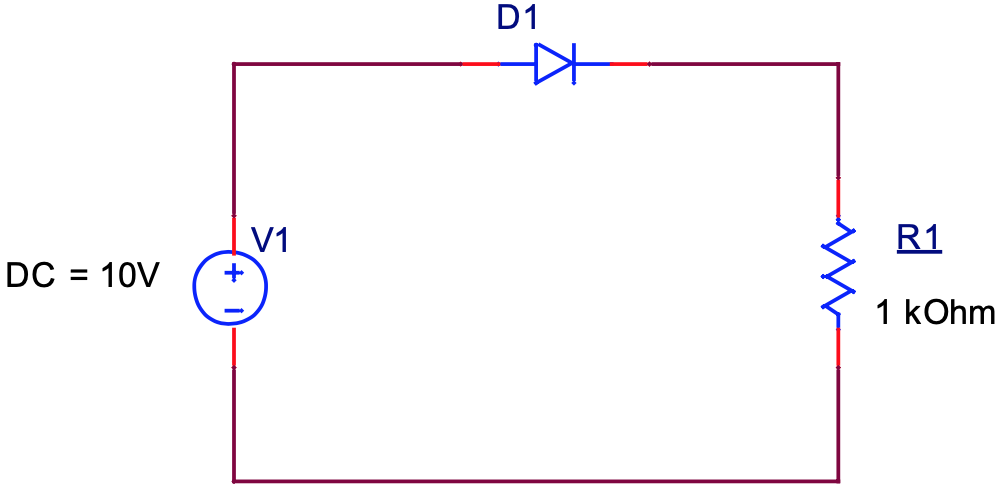
\includegraphics[scale=0.3,angle=0]{diodi_es1.png}
    \end{figure}
    \\Il circuito è costituito da una sola \textbf{maglia}, il che significa che nel circuito scorre una sola corrente che è la stessa per tutti i dispositivi che lo compongono. Considerando i due nodi alle due estremità del generatore di tensione, la differenza di potenziale tra questi due nodi è esattamente quella erogata dal generatore, cioè $V_{DC} = 10\,V$. Questa tensione deve essere uguale alla tensione tra le due estremità del cammino passante per il diodo $D_1$ e la resistenza $R_1$ (avente una tensione ai suoi estremi indicata con $V_{R_1}$):
    \begin{equation}
        V_{DC} = V_{D_1} + V_{R_1}
        \label{tensione_circuito1_1}
    \end{equation}
    Osservando ora $D_1$ si nota che è polarizzato direttamente perché sull'anodo è applicato il potenziale positivo del generatore di tensione e sul catodo un potenziale negativo. Si sa che la tensione di un diodo polarizzato direttamente può essere considerata all'incirca constante e dipende dalla tipologia di diodo: per un diodo al silicio si può supporre una tensione di circa $0,7\,V$, per un diodo LED la tensione varia in base al colore emesso.\\Supponendo che $D_1$ sia un LED rosso si ottiene $V_{D_1} = 1,5\,V$, quindi la \eqref{tensione_circuito1_1} diventa:
    \begin{equation}
        10\,V = 1,5\,V + V_{R_1}
        \label{tensione_circuito1_2}
    \end{equation}
    Infine, $R_1$ è una resistenza quindi vale la legge $V_{R_1} = R_{1} \cdot I$, dove \textit{I} è la corrente che scorre nella resistenza che è la stessa che scorre nel diodo e quella che esce dal generatore, cioè è la corrente dell'intero circuito. Dunque la \eqref{tensione_circuito1_2} diventa:
    \begin{equation*}
        10\,V = 1,5\,V + (R_1 \cdot I)
    \end{equation*}
    Si può quindi calcolare la corrente che scorre nel circuito come:
    \begin{equation*}
        I = \frac{10\,V - 1,5\,V}{R_1} = \frac{10\,V - 1,5\,V}{1000\,\Omega} = 8,5 \cdot 10^{-3}\,A
    \end{equation*}
    \newpage
    \item Calcolare $\frac{V_{out}}{Light_{in}}$ per il seguente circuito:
    \begin{figure}[ht]
        \centering
        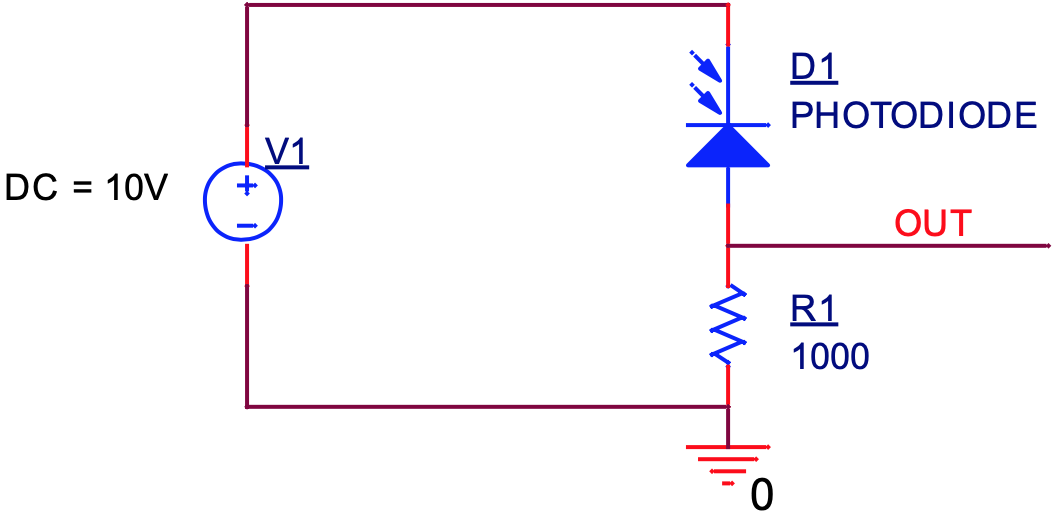
\includegraphics[scale=0.3,angle=0]{diodi_es2.png}
    \end{figure}
    \\Si sa che il fotodiodo lavora polarizzato inversamente e, se arriva un fotone, scorre una corrente che va dal catodo all'anodo. Consultando il datasheet del fotodiodo è possibile sapere la corrente che esce dal fotodiodo $I_{out}$ in rapporto ad una certa densità di potenza luminosa in ingresso $P_{in}$ generalmente espressa in $mWcm^{-2}$. Si prende per esempio una corrente uscente dal fotodiodo di $1 \frac{mA}{mWcm^{-2}}$. Questa corrente passa attraverso la resistenza $R_1$, il che significa che:
    \begin{equation*}
        V_{out} = R_1 \cdot I = 1000\,\Omega \cdot 1\,\frac{mA}{mWcm^{-2}} = 1\,\frac{V}{mWcm^{-2}}
    \end{equation*}
    Sapendo che in media la luce solare è di $0,15\,mWcm^{-2}$, la tensione massima in uscita sarà circa tra $0,1\,mV$ e $0,15\,mV$. Per fa sì che il circuito conservi un comportamento lineare $V_{out}$ deve essere piccola, perché la tensione inversa applica al fotodiodo è la tensione del generatore $V_{DC} = 10\,V$ meno la tensione che cade ai capi della resistenza $R_1$. Quindi minora sarà la tensione della resistenza e meno bias negativo ci sarà sul fotodiodo che andrà a modificare la caratteristica del foto rilevatore. Questo circuito risulta quindi essere poco sensibile e poco lineare perché la polarizzazione del fotodiodo cambia con la corrente di uscita che va a modificare la sua linearità. Per migliorarlo si considera il circuito nell'esercizio successivo.
    \item Calcolare $\frac{V_{out}}{Light_{in}}$ nel seguente circuito:
    \begin{figure}[h]
        \centering
       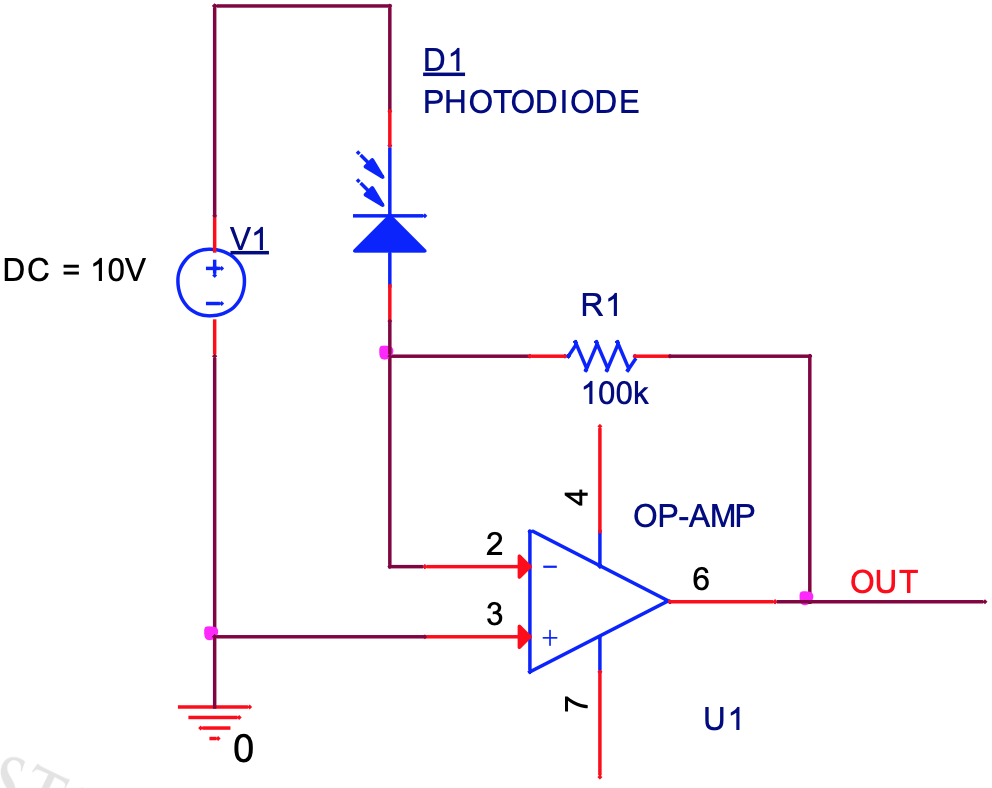
\includegraphics[scale=0.3,angle=0]{diodi_es3.png}
    \end{figure}
    \\L'amplificatore operazionale è composto da una uscita rappresentante l'uscita di un generatore di tensione e da due ingressi, uno in positivo e uno in negativo. Quando si chiude il circuito in retroazione con un'apposita rete (in questo caso la resistenza $R_1$) sono valide due equazioni:
    \begin{enumerate}
        \item $V_{-} = V_{+}$: la tensione dei due terminali 2 e 3 è la stessa; non c'è differenza di potenziale perché l'amplificatore operazionale in anello aperto (cioè eliminando la retroazione data dalla resistenza $R_1$) amplifica con un valore ideale infinito la differenza tra i due ingressi 2 e 3 esponendola in uscita. Quando invece l'amplificatore viene chiuso in retroazione tramite $R_1$, l'uscita si stabilizza e valgono queste due equazioni.
        \item $I_{-} = I_{+} = 0$: i due nodi di ingresso + e - non assorbono corrente
    \end{enumerate}
    Sfruttando queste due equazioni è possibile risolvere il circuito. L'ingresso positivo 3 dell'amplificatore operazionale ha un valore di tensione fisso che in questo caso è $V_{3} = 0\,V$, inoltre sempre nel piedino 3 non scorre corrente cioè $I_{3} = 0\,A$. Dalla prima equazione segue che $V_{2} = 0\,V$. Il fotodiodo, trovandosi tra la $V_{+}$ del generatore e la $V_{2}$ dell'amplificatore operazionale ha una tensione inversa $V_{D} = V_{DC} = 10\,V$ indipendentemente dalla corrente che scorre nel fotodiodo perché tale corrente non può andare nel piedino 2 perché l'amplificatore operazionale non accetta corrente in ingresso (infatti $I_{-} = 0\,A$), dunque per costruzione del circuito andrà nel ramo contente la resistenza in retroazione $R_1$ andando quindi verso l'uscita dell'amplificatore. Per calcolare $V_{out}$ devo risalire ad un punto di potenziale noto che è il nodo tra il fotodiodo e $R1$ (corrisponde anche al nodo sottostante tra il fotodiodo e il piedino 2) in cui si sa che $V = V_{2} = 0\,V$, dunque $V_{out} = V_{2} \,-\, ( R_1 \cdot I_{D}) = 0\,V \,-\, (100k\,\Omega \cdot I_{D}) = - 100k\,\Omega \cdot I_{D}$. Ma $I_{D}$, come nell'esercizio precedente si prendere pari a $1 \frac{mA}{mWcm^{-2}}$, dunque:
    \begin{equation*}
        V_{out} = - 100k\,\Omega \cdot 1 \frac{mA}{mWcm^{-2}} = - 100\,\frac{V}{mWcm^{-2}}
    \end{equation*}
    Questo circuito, rispetto a quello nell'esercizio precedente, guadagna circa 100 volte. Sapendo che in media la luce solare è di $0,15\,mWcm^{-2}$, la tensione massima in uscita sarà circa tra $-10\,V$ e $-15\,V$. Il meno è dovuto al fatto che si sta utilizzando l'amplificatore operazionale in \textit{configurazione invertente}. Per risolvere questo problema si può aggiungere un secondo stadio in uscita all'amplificatore che guadagna a sua volta $-1\,V$ così da riportare la tensione in positivo, oppure al posto di porre $V_{3} = V_{+} = 0\,V$ si possono mettere due resistenze tra generatore e il piedino 3 eliminando la messa a terra così da creare una tensione $V_{offset}$ in modo da ottenere $V_{2} = V_{3} = V_{offset}$ e  $V_{D} = V_{DC} - V_{offset}$ e l'uscita sarà $V_{out} = V_{offset} - qualcosa$. Si può fare in modo che alla fine torni positiva e alla massima intensità luminosa l'uscita arrivi a $0\,V$. Il vantaggio di questo circuito è che, indipendentemente dalla tensione di uscita, il nodo dell'anodo del fotodiodo rimane ad una tensione costante e quindi il fotodiodo rimane polarizzato ad una tensione costante non soffrendo di non linearità.
\end{enumerate}
\chapter{Esercizi BJT}
\begin{enumerate}
    \item Calcolare la tensione di uscita $V_{out}$ del seguente circuito:
    \begin{figure}[h]
        \centering
       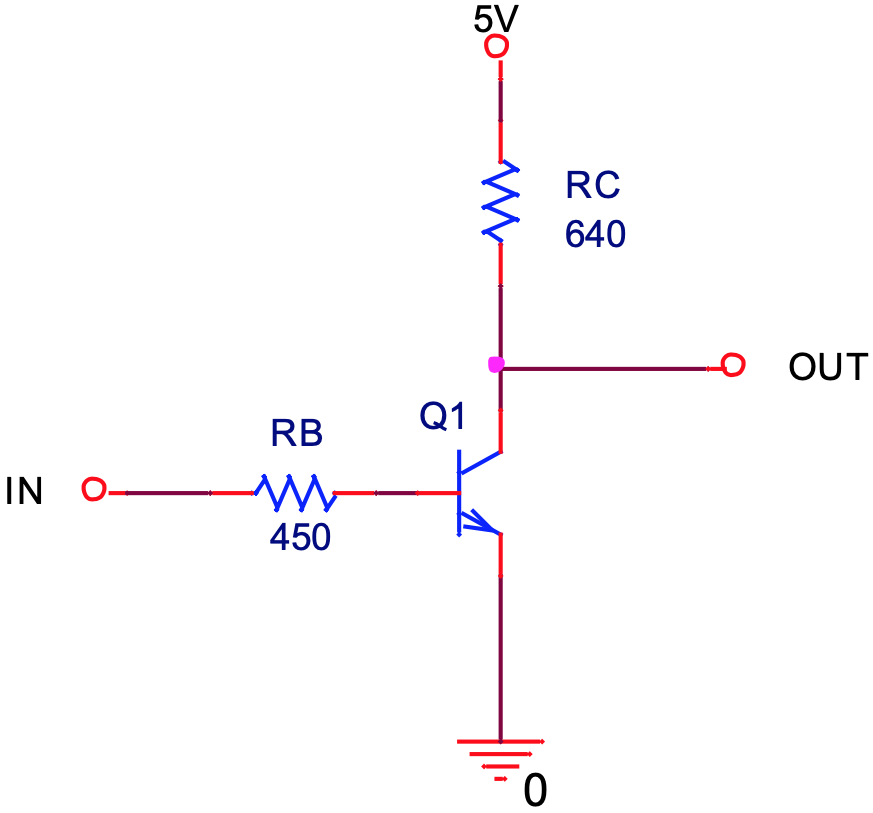
\includegraphics[scale=0.3,angle=0]{bjt_es1.png}
    \end{figure}
    \\Si sa che il guadagno in corrente di $Q_1$ vale $h_{fe} = 50$ e che la tensione in ingresso (applicata sul nodo IN) vale $V_{in} = 1,15\,V$. La tensione di uscita si definisce considerando il fatto che nella resistenza di collettore $R_{c}$ scorre la corrente di collettore $I_{c}$ e tutto questo genera una tensione, dunque:
    \begin{equation*}
        V_{out} = V_{c} - (R_{c} \cdot I_{c}) = 5\,V - (R_{c} \cdot I_{c})
    \end{equation*}
    Si deve stabilire quanto vale $I_{c}$. Siccome $V_{in} = 1,15\,V$  è maggiore di $0,6 - 0,7\,V$, la giunzione tra la base e l'emettitore è polarizzata \textit{direttamente} e questo comporta che il transistor si trova o in saturazione oppure in regione attiva diretta. Supponendo che si trovi in regione attiva diretta la corrente del collettore varrà $I_{c} = h_{fe} \cdot I_{b}$ quindi:
    \begin{equation}
        V_{out} = V_{c} - [R_{c} \cdot (h_{fe} \cdot I_{b})]
        \label{v_out}
    \end{equation}
    e $V_{out}$ (la tensione del collettore) dovrà essere maggiore di $0,2\,V$. Si può quindi verificare a posteriori se l'ipotesi di regione attiva diretta è verificata o meno. Sapendo che $V_{in} = 1,15\,V$ e $V_{b} \approx 0,7\,V$, la tensione che cade sulla resistenza di base $R_{b}$ vale
    \begin{equation*}
        V_{R_{b}} = 1,15\,V - 0,7\,V = 0,45\,V = 450\,mV
    \end{equation*} 
    dunque la corrente di base è la corrente che scorre nella resistenza di base $R_b$ e vale
    \begin{equation*}
        I_{b} = I_{R_{b}} = \frac{V_{R_b}}{R_b} = \frac{0,45\,V}{450\,\Omega} = 1\cdot 10^{-3}\,A = 1\,mA
    \end{equation*}
    A questo punto sfruttando la \eqref{v_out} si può calcolare la tensione di uscita:
    \begin{equation*}
        V_{out} = 5\,V - [640\,\Omega \cdot (50 \cdot 1\cdot 10^{-3}\,A)] = -\,27\,V
    \end{equation*}
    ma questo è impossibile perché in attiva diretta $V_{out}$ deve essere maggiore di $0,2\,V$ quindi l'ipotesi fatta di trovarsi in regione attiva diretta non è valida: il transistor si trova in \textit{saturazione}. Trovandosi in saturazione si ottiene:
    \begin{equation*}
        V_{out} = V_{c-sat} = 0,2\,V
    \end{equation*}
    Si può anche calcolare la corrente di saturazione che scorre dal collettore all'emettitore e che è minore della corrente che si avrebbe in attiva diretta $I_{c} = h_{fe} \cdot I_{b} = 50 \cdot 10^{-3}\,A$ come
    \begin{equation*}
        I_{c} = \frac{V_{R_c}}{R_{c}} = \frac{5\,V - 0,2\,V}{640\,\Omega} = 7,5\,mA
    \end{equation*}
    quindi è solo 7 volte superiore alla corrente di base $I_{b} = 1\,mA$.
    \item Se la resistenza del collettore nel circuito precedente vale $R_{c} = 50\,\Omega$, ci si aspetta che cadrà meno tensione su $R_c$ e quindi sarà più facile utilizzare il transistor in regione attiva. La corrente di base resta invariata, dunque $I_{b} = 1\,mA$.  Supponendo che il transistor si trovi in regione attiva diretta la corrente del collettore varrà ancora
    \begin{equation*}
        I_{c} = h_{fe} \cdot I_{b} = 50 \cdot 1 \cdot 10^{-3}\,A = 50\,mA
    \end{equation*}
    e al tensione di uscita sarà:
    \begin{equation*}
        V_{out} = V_{ce} = V_{c} - (R_{c} \cdot I_{c}) = 5\,V - (50\,\Omega \cdot 50\,mA) = 2,5\,V
    \end{equation*}
    che è maggiore di $0,2\,V$ quindi il transistor permane effettivamente in regione \textit{attiva diretta}, la tensione di collettore è funzione della corrente d'ingresso e di conseguenza la tensione di uscita è funzione \textit{lineare} della corrente di collettore quindi della corrente di base. Si ha effettivamente un dispositivo controllato in corrente che è un amplificatore di corrente e di tensione con guadagno in corrente $h_{fe}$ e guadagno in tensione $-\frac{R_c}{R_b} \cdot h_{fe}$ ricavabile dal fatto che, trascurando $V_{c} = 5\,V$, la tensione di uscita vale:
    \begin{align*}
        V_{out} &= -\,R_{c} \cdot I_{c} = -\,R_{c} \cdot h_{fe} \cdot I_{b}\\ &= -\,R_{c} \cdot h_{fe} \cdot \frac{V_{in - 0,7\,V}}{R_{b}}\\
        &= -\frac{R_c}{R_b} \cdot h_{fe} \cdot (V_{in} - 0,7\,V)
    \end{align*}
    \item Calcolare il valore delle resistenze $R_1$ e $R_2$ nel seguente circuito in modo da accendere il LED in rosso con una corrente di $20\,mA$ e il transistor $Q_1$ sia in saturazione:
    \begin{figure}[h]
        \centering
       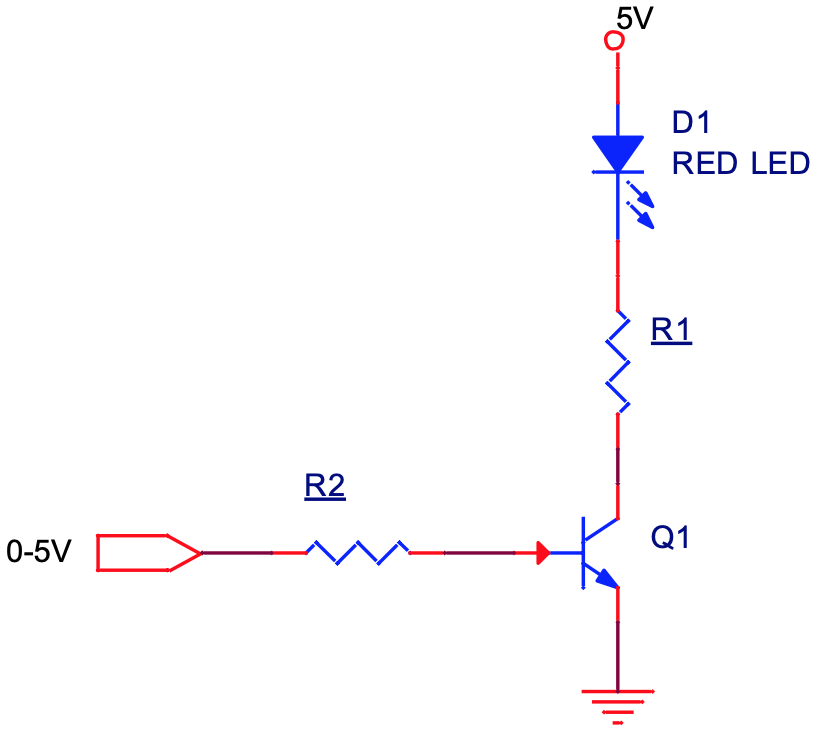
\includegraphics[scale=0.3,angle=0]{bjt_es2.png}
    \end{figure}
    \\Si sa che $Q_1$ è un BJT di tipo \textit{npn} con guadagno in corrente $h_{fe} = 50$. La tensione della base del transistor quando il led è spento è di $0\,V$ e quando si accende è di $5\,V$. Quando si vuole accendere il LED e quindi usare il transistor come interruttore (come un dispositivo digitale), quest'ultimo deve essere tenuto nella regione di \textit{cutoff} o di \textit{saturazione} senza mai mandarlo in attiva diretta perché in quella regione funzionerebbe come un amplificatore, mentre in saturazione è un dispositivo non lineare; cioè è come se fosse un normale interruttore chiuso con tensione ai capi dell'interruttore è $=0,2\,V$. Non ci sarebbe nessun problema ad usare il transistor in attiva diretta o inversa ma il guadagno in corrente $h_{fe}$ non è facilmente predicibile e non è molto stabile (sul datasheet ne vengono indicati il valore minimo, massimo e medio) sia a livello di parametro costruttivo sia a livello di temperatura (se il transistor si scalda o raffredda $h_{fe}$ varia). Se si deve usare il transistor per accendere un LED e far scorrere una corrente nota, come in questo caso, si deve usarlo in \textit{saturazione} perché si è certi che la tensione di saturazione è $0,2\,V$ mentre in regione lineare non si ha la certezza che il suo guadagno in corrente sia 50. Per usarlo in saturazione si deve fare in modo che:
    \begin{equation*}
        I_{c} = 20\,mA < h_{fe} \cdot I_{b}
    \end{equation*}
    ovvero che, per $h_{fe_{min}} = 50$
    \begin{equation}
        I_{b} > \frac{20\,mA}{h_{fe}} = \frac{20\,mA}{50} = 0,4\,mA
        \label{condizione_r2}
    \end{equation}
    Trovandosi in saturazione la giunzione tra la base e l'emettitore è polarizzata \textit{direttamente} (perché l'emettitore è a massa e la tensione della base è positiva e vale $5\,V$), quindi $V_{b} = 0,7\,V$. Volendo accendere il LED, al capo sinistro di $R_2$ si una tensione di $5\,V$, quindi
    \begin{equation*}
        V_{R_2} = 5\,V - 0,7\,V = 4,3\,V
    \end{equation*}
    Dovendo valere $V_{R_2} = R_{2} \cdot I_{b}$ con $I_{b} > 0,4\,mA$ secondo la \eqref{condizione_r2}, si ottiene:
    \begin{equation*}
        R_{2} \leq \frac{4,3\,V}{0,4\,mA} = 11\,k\Omega
    \end{equation*}
    Se il transistor è in saturazione, la tensione del collettore è $V_{c} = 0,2\,V$. Sapendo che al capo in alto è applicata una tensione di $5\,V$ e che nel ramo sono presenti la resistenza $R_1$ e il diodo $D_1$, deve valere:
    \begin{equation}
        V_{R_1} + V_{D_1} = 5\,V - 0,2\,V = 4,8\,V
        \label{condizione_r1}
    \end{equation}
    Inoltre, si vuole che il LED emetta luce rossa, quindi $V_{D_1} = 1,5\,V$. Sostituendo nella \eqref{condizione_r1} si ottiene
    \begin{equation*}
        V_{R_1} = 4,8\,V - V_{D_1} = 4,8\,V - 1,5\,V = 3,3\,V
    \end{equation*}
    Sapendo infine che il LED e $R_1$ sono attraversati da una corrente di $20\,mA$ e dovendo valere $V_{R_1} = R_{1} \cdot I_{R_1}$ si ottiene
    \begin{equation*}
        R_{1} = \frac{V_{R_1}}{I_{R_1}} = \frac{3,3\,V}{20\,mA} = 165\,\Omega
    \end{equation*}
    Se per esempio si avesse $h_{fe} = 50$ non cambierebbe niente perché si sta lavorando in saturazione, quindi rimarrebbe sia $V_{ce} = 0,2\,V$ sia $V_{R_1} = 3,3\,V$. Invece per $h_{fe} = 10$ si passerebbe in regione lineare e la corrente che scorre nel LED sarà diversa.
\end{enumerate}
\chapter{Esercizi MOS}
\begin{enumerate}
    \item Valutare il valore del parametro \textit{K} in base alle seguenti curve:
    \begin{figure}[h]
        \centering
       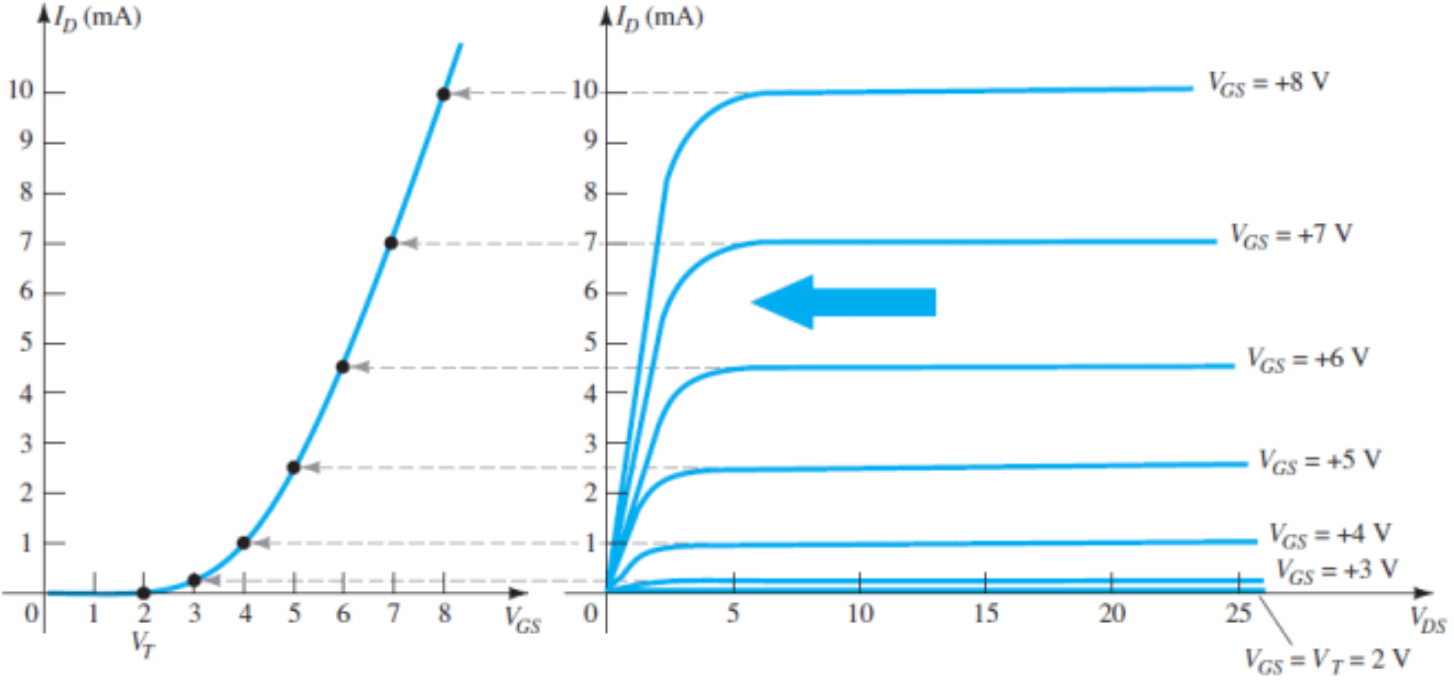
\includegraphics[scale=0.4,angle=0]{n_mos_es1.png}
    \end{figure}
    \\Si sa che la corrente di saturazione è definita dall'equazione
    \begin{equation}
        I_{d-sat} = K(V_{gs} - V_{t})^2
        \label{sat}
    \end{equation}
    Nel caso in questione la tensione limite è già fornita e si sa che $V_{t} = 2\,V$. A partire dal grafico di sinistra, che ha per ascissa la tensione $V_{gs}$ e per ordinata la corrente di saturazione $I_{d-sat}$, è possibile determinare la corrente di saturazione corrispondente ad un determinato valore della tensione di gate. Dalla \eqref{sat}, che è diventata una relazione ad una sola incognita, si può quindi ricavare il valore della costante \textit{K} come:
    \begin{equation*}
        K = \frac{I_{d-sat}}{(V_{gs} - V_{t})^2}
    \end{equation*}
    Per esempio, per $V_{gs} = 8\,V$ corrisponde una corrente di saturazione $I_{d-sat} = 10\,mA$ dunque $K = 2,8 \cdot 10^{-4}$.
    
    Se $V_{t}$ non fosse nota, si avrebbero due incognite nella \eqref{sat}. Per poter risolvere il problema si dovrebbe quindi risolvere un sistema di due equazioni in due incognite sfruttando la definizione di $I_{d-sat}$ e le coppie $(V_{gs}$, $I_{d}$) ricavabili nel grafico di destra. Per esempio, per $V_{gs} = 4\,V$ corrisponde una corrente di saturazione $I_{d-sat} = 1\,mA$ e, come detto prima, per $V_{gs} = 8\,V$ corrisponde una corrente di saturazione $I_{d-sat} = 10\,mA$ dunque:
    \begin{equation*}
    \left\{
    \begin{array}{l}
    10\,mA = K(8\,V - V_{t})^2\\
    1\,mA = K(4\,V - V_{t})^2
\end{array}\right.
\end{equation*}

\end{enumerate}
\end{appendices}
\end{document}
